\chapter{Results}

\section{Employing the Pipeline and  Evaluation}\label{section:employing-proposed-pipeline}
Total of 11 experiments (7 wild type sleep and 4 sleep-deprived) and their annotations are split as 10 training experiments and 1 test experiment for all combinations.
We report results and evaluate each split and demonstrate varying performance for different splits.

Our pipeline starts with the feature extraction stage, where raw tracking data generated by DeepLabCut is used to generate meaningful behavioral representations.
Body parts used to extract features are proboscis, haltere, thorax, head (left and right), leg joints (left and right).
We use oriented pose vales for body parts with left and right counterparts, as described in the Section~\ref{section:oriented-pose-values}.
In order to detect occluded body parts, we set the low confidence score threshold to $0.075$.
Moving median window size $\tau$ is $15$ frames, ($0.5$ seconds) and threshold $\tau$ set to $15$ microns. If the position of a body part exceeds the median of the window centered around it by $\tau$, it is marked as occluded, as described in Section~\ref{section:detecting-occlusions}
Linear interpolation is used for imputation of marked frames.
After that, firstly, a median filter of size $6$ frames, and then a boxcar filter of size $6$ frames is applied to reduce the tracking noise and smooth the signal, without smoothing behaviors exhibited by rapid movements.
Aligning different orientations and transforming the frames to be egocentric did not result in performance improvement in our case, hence, we continued without making frames egocentric.

Then, we computed snapshot features and gradient features as described in Section~\ref{section:spatiotemporal-fetaures}, and given in the Table~\ref{table:spatiotemporal-features}.
In order to generate postural dynamics, wavelet transformation is applied to snapshot features at $20$ different frequency channels dyadically spaced between $1$ Hz and $20$ Hz (see Equation~\ref{equation:dyadically-spaced-spectrum} for determining spectrum frequencies).
Then different timescales are normalized as given in Equation~\ref{equation:wavelet-normalization}.
After flattening and $\textnormal{L}_1$ frame normalization, we ended up with a $13 \times 20 = 260$ dimensional behavioral representation matrix $\V{\hat{W}}$.
Similarly, for gradient features, moving mean values are computed for a single timescale which is $33$ milliseconds, resulting in $9 \times 1 = 9$ dimensional behavioral representation matrix $\V{\hat{M}}^\mu$, which is only used for experiment outlining and constructing $\Dormancy$ set.

\begin{table}[htb!]
	\begin{adjustbox}{width=1\textwidth}
		\begin{tabular}{c l l}
			\toprule
			                                         & \multicolumn{1}{c}{\textbf{Snapshot Features}} & \multicolumn{1}{c}{\textbf{Gradient Features}} \\
			\cmidrule(lr){2-2}\cmidrule(lr){3-3}
			\multirow{7}{*}{Distance between}        & haltere and origin                             & head and proboscis                             \\
			                                         & proboscis and origin                           & thorax and proboscis                           \\
			                                         & thorax and origin                              & thorax and origin                              \\
			                                         & head and proboscis                             &                                                \\
			                                         & haltere and thorax                             &                                                \\
			                                         & (average) leg joints and origin                &                                                \\
			                                         & (average) leg joints and thorax                &                                                \\
			\cmidrule(lr){2-2}\cmidrule(lr){3-3}
			\multirow{3}{*}{Cartesian components of} & haltere                                        & head                                           \\
			                                         & head                                           & proboscis                                      \\
			                                         & thorax                                         & thorax                                         \\
			\bottomrule
		\end{tabular}
	\end{adjustbox}
	\caption{Computed spatio-temporal features. \label{table:spatiotemporal-features}}
\end{table}

After constructing behavioral representation matrices, the experiment outlining stage of our pipeline takes place.
Here reported recall scores are for the frame set $\MicroActivity$, and it is desired to achieve high recall scores, except for the ``quiescent and other'' category.
We evaluate both unsupervised and supervised approaches, recall scores and the accuracy is given in the Figure~\ref{figure:outlining-performance}.

\begin{figure}[htb!]
	\centering
	\begin{subfigure}[b]{0.495\linewidth}
		\centering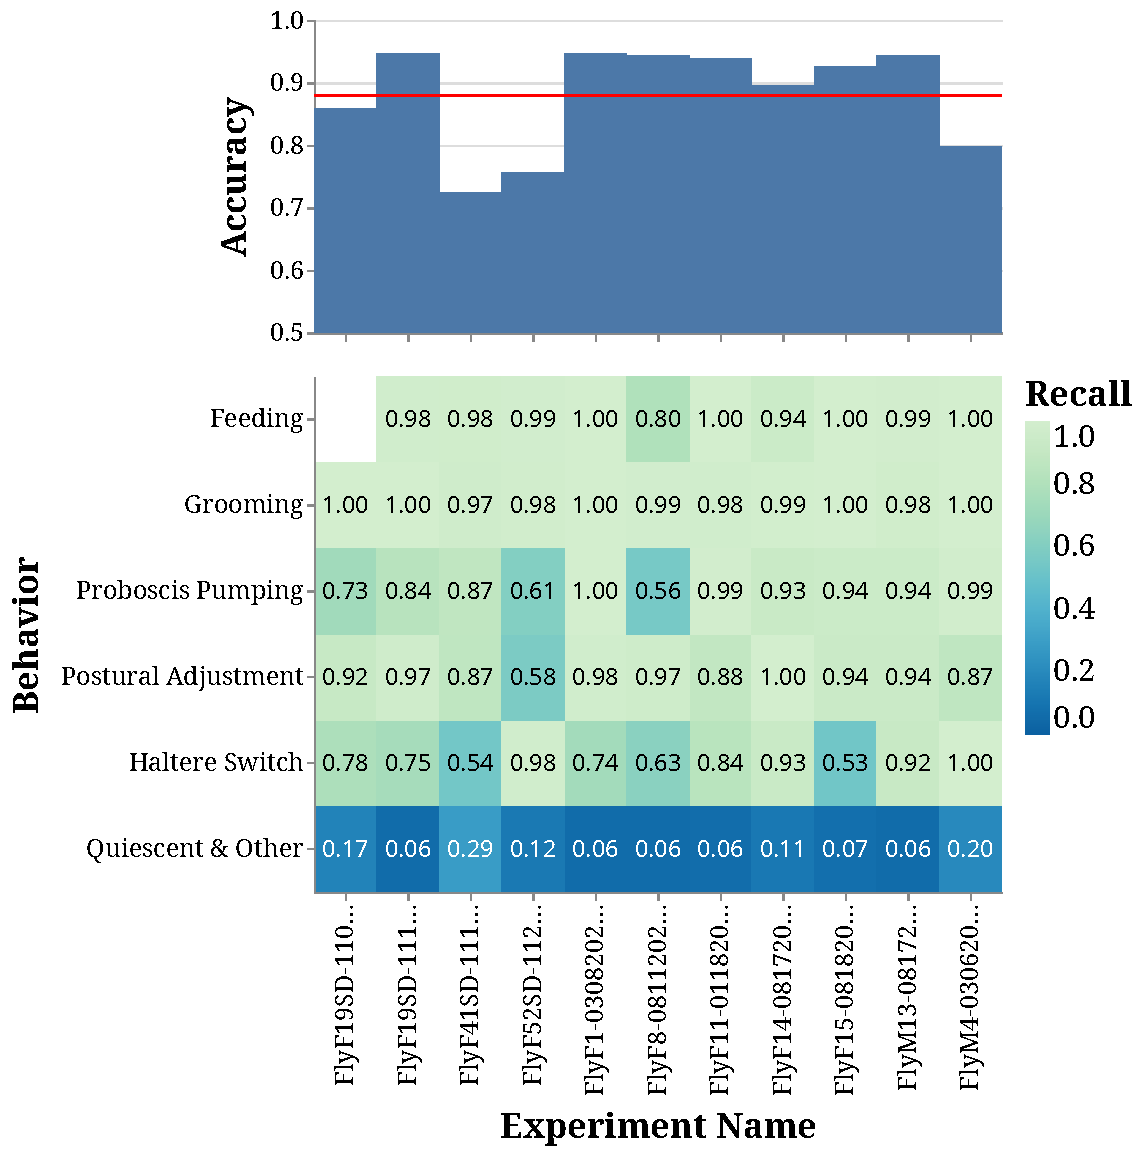
\includegraphics[width=\linewidth]{figures/OutliningPerformance-Supervised.pdf}
		\caption{Supervised detection.}
	\end{subfigure}%
	\hfill
	\begin{subfigure}[b]{0.495\linewidth}
		\centering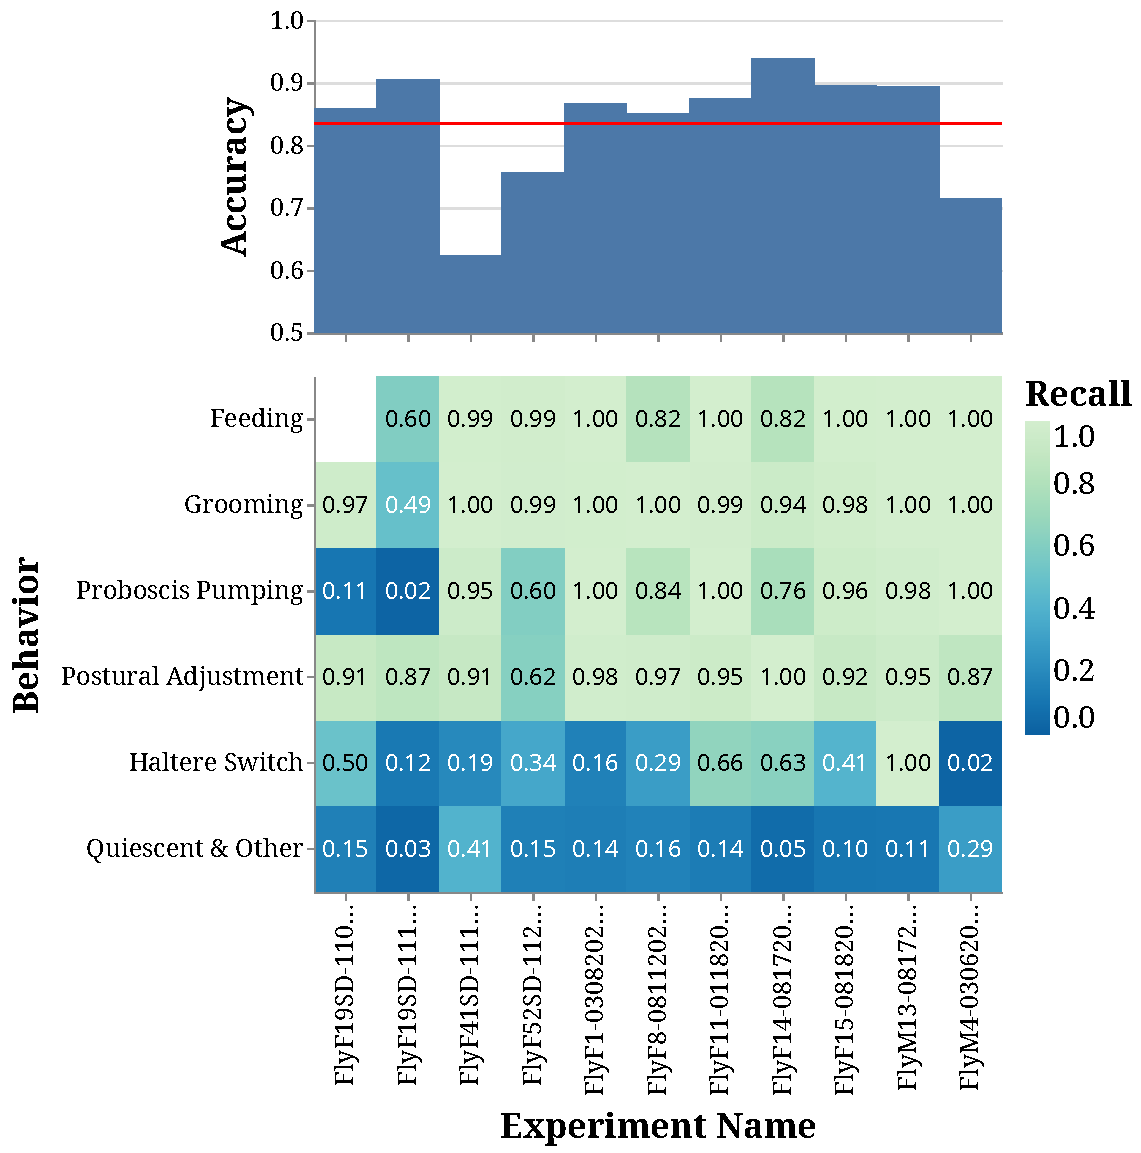
\includegraphics[width=\linewidth]{figures/OutliningPerformance-Unsupervised.pdf}
		\caption{Unsupervised detection.}
	\end{subfigure}%
	\caption[Performance summary of experiment outlining and micro-activity detection.]{Performance summary of experiment outlining and micro-activity detection.
		The red line indicates the macro average of accuracy scores achieved for each split.
		High recall scores are desired for behavioral categories, as opposed to quiescent frames.
		Supervised and unsupervised detections are given respectively in the left subfigure and in the right subfigure. \label{figure:outlining-performance}}
\end{figure}

For unsupervised experiment outlining, the threshold $c$ is set to the decision boundary $\lambda_1$ of two Gaussian components for construction of the $\Dormancy$ set.
Similarly, thresholds $c_i$ for each $\V{u}_i$ value are the first decision boundaries of $3$ Gaussian components, sorted by their means.
Resulting detection performance is quite poor for switch-like behavior of haltere, since this behavior occurs very subtly, and it is similar to quiescent frames.
8 out of 11 splits, has recall score less than $0.5$.
Also, recall scores for two of the sleep-deprived experiment splits (FlyF19SDs) are below $0.15$, which makes it impossible to proceed with a successful mapping.

In the supervised approach, a random forest of decision trees \citep{breiman_random_2001} is utilized with $10$ estimators, where the maximum depth of each tree is $5$ and the criterion is Gini impurity.
For grooming, recall is always greater than $0.97$, which implies that we do not lose an insignificant amount of annotated frames.
Similarly, the recall score of feeding drops below $0.95$ only once.
For proboscis pumping, 6 out of 11 splits have recall score greater than $0.9$, and performance is relatively poor for two splits ($0.61$ and $0.56$ recall).
Again, haltere switch is the most challenging behavioral category, but recall is often greater than $0.75$ as opposed to unsupervised approach.
Considering its superior performance over unsupervised approach, we proceed to behavior mapping by employing supervised outlining.

After experiment outlining, the next stage is the behavior mapping, where the frames in the set $\MicroActivity$ are mapped to behavioral categories.
First step is computation of behavioral embeddings.
The semi-supervised pair embeddings described in the Section~\ref{section:pair-embeddings} computed for each annotated and unannotated experiment pair.
We set the embedding space dimension to 2, which $260$ dimensional behavioral representation matrix $\V{\hat{W}}$ is reduced to.
Number of neighbors parameter of UMAP is set to $75$, minimum distance parameter is determined as $0$, and the distance metric is Hellinger distance (Equation~\ref{equation:hellinger-distance}).

Then, with the generated behavioral embeddings, nearest neighbors analysis is performed to assign behavioral scores to unannotated frames.
In each semi-supervised embedding, we computed $25$ nearest annotated neighbors of the frames, and contributions of the neighbors are weighted disproportional to its distance, using the Euclidean distance, as formally given in the Equation~\ref{equation:nn-weights}.
After that, weights are normalized with the $\log_2$ number of occurrences of behavioral category of contributing neighbors, and then $\textnormal{L}_1$ normalized to make behavioral weights sum up to $1$ (see Equation ~\ref{equation:behavioral-weight-occurence-normalization}, ~\ref{equation:behavioral-weight-activation}). Finally, we summed each behavioral weight, obtained from a different ``view'' (i.e., annotated experiment), and $\textnormal{L}_1$ normalized again to end up with the final behavioral score values.

\begin{figure}[htb!]
	\centering
	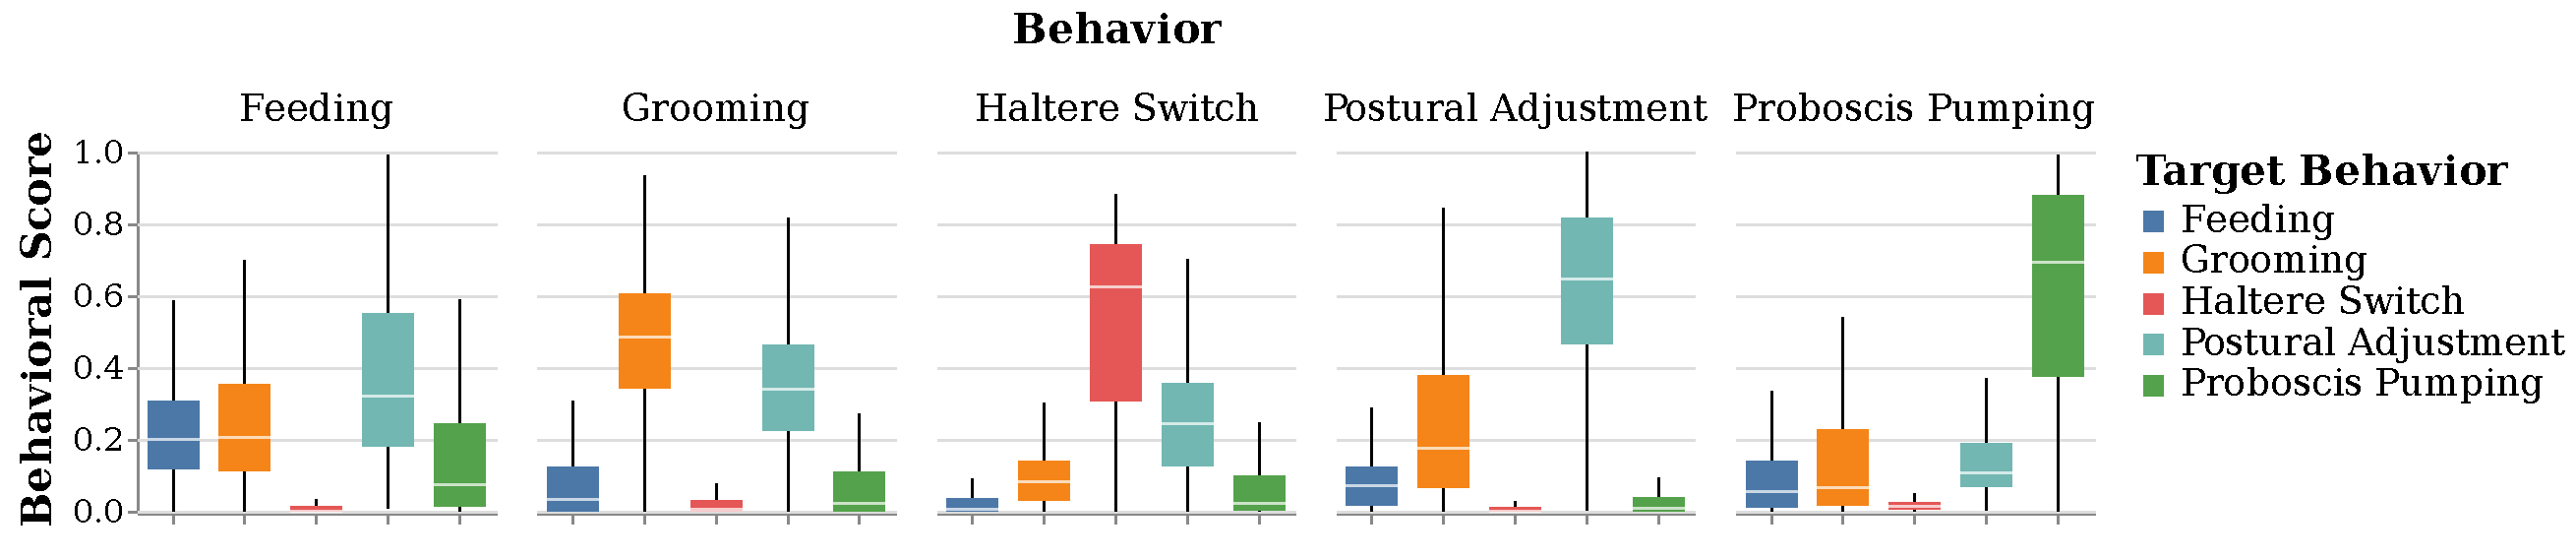
\includegraphics[width=\linewidth]{figures/BehavioralScoresDistributions_perBehavior.pdf}
	\caption[Distributions of behavioral score values of each behavioral category for all splits.]{Distributions of behavioral score values of each behavioral category for all splits.
		Each box-plot column demonstrates the behavioral score distributions of target behaviors for the corresponding annotation.\label{figure:behavioral-score-distributions}}
\end{figure}

Resulting score vectors are used for classification and also utilized as confidence scores.
In the Figure~\ref{figure:behavioral-score-distributions}, behavioral score distribution for each category is given for all splits together.
Except for the feeding category, median score of the correct target behavioral category is greater than $0.5$.
Grooming and postural adjustment are the second most similar target behavior for each other, as expected.
When the grooming behavior is short, it becomes more similar to short duration moving and postural adjustment behavior.
Behavioral scores also helpful for revealing similarities and dissimilarities between behavioral categories, and can be helpful for determining spatio-temporal feature set.
Although we normalized behavioral weights with number of occurrences, which favors the relatively short duration and rare switch-like haltere behavior, we can see that its target behavior score does not exceed $0.1$ for wrong categories.
Compared to other behaviors, feeding has the poorest performance, with median correct score $0.2$.
Postural adjustment category wrongly has the highest median score for feeding.
Frames with feeding behavior annotation often misidentified as postural adjustment, grooming, and proboscis pumping.
As proboscis movement is common both for feeding and proboscis pumping, confusion with the proboscis pumping is expected for feeding.

\begin{figure}[htb!]
	\centering
	\begin{subfigure}[b]{0.99\linewidth}
		\centering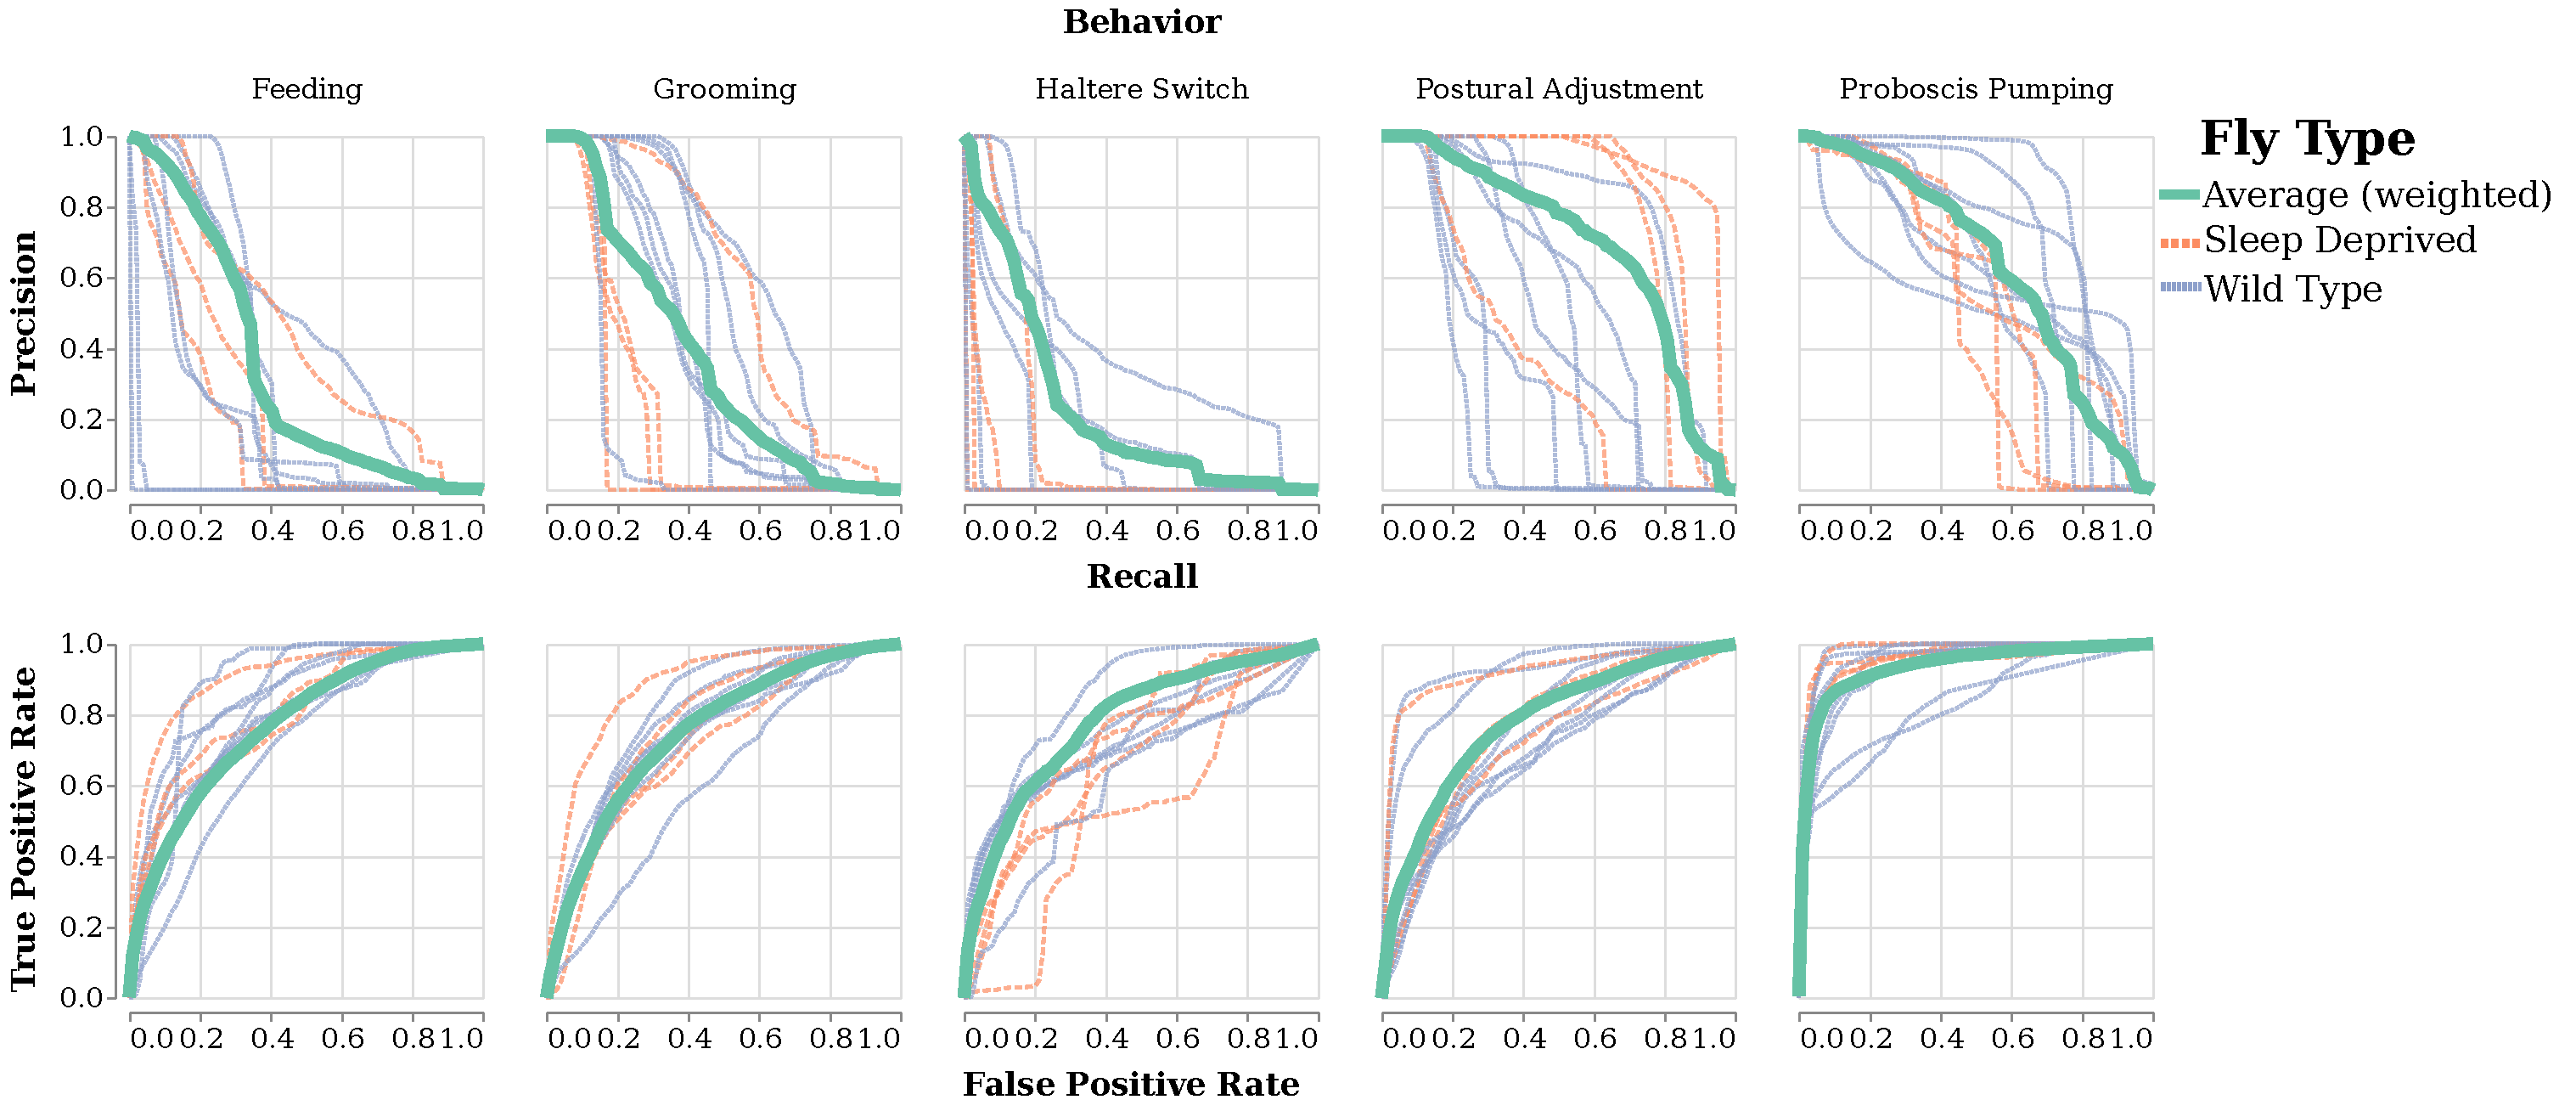
\includegraphics[width=\linewidth]{figures/PRC_ROC-DActfiltered.pdf}
		\caption{ROC and precision-recall curves for frames detected as micro-activity. \label{figure:ROC-PRC-Act}}
	\end{subfigure}%

	\begin{subfigure}[b]{0.99\linewidth}
		\centering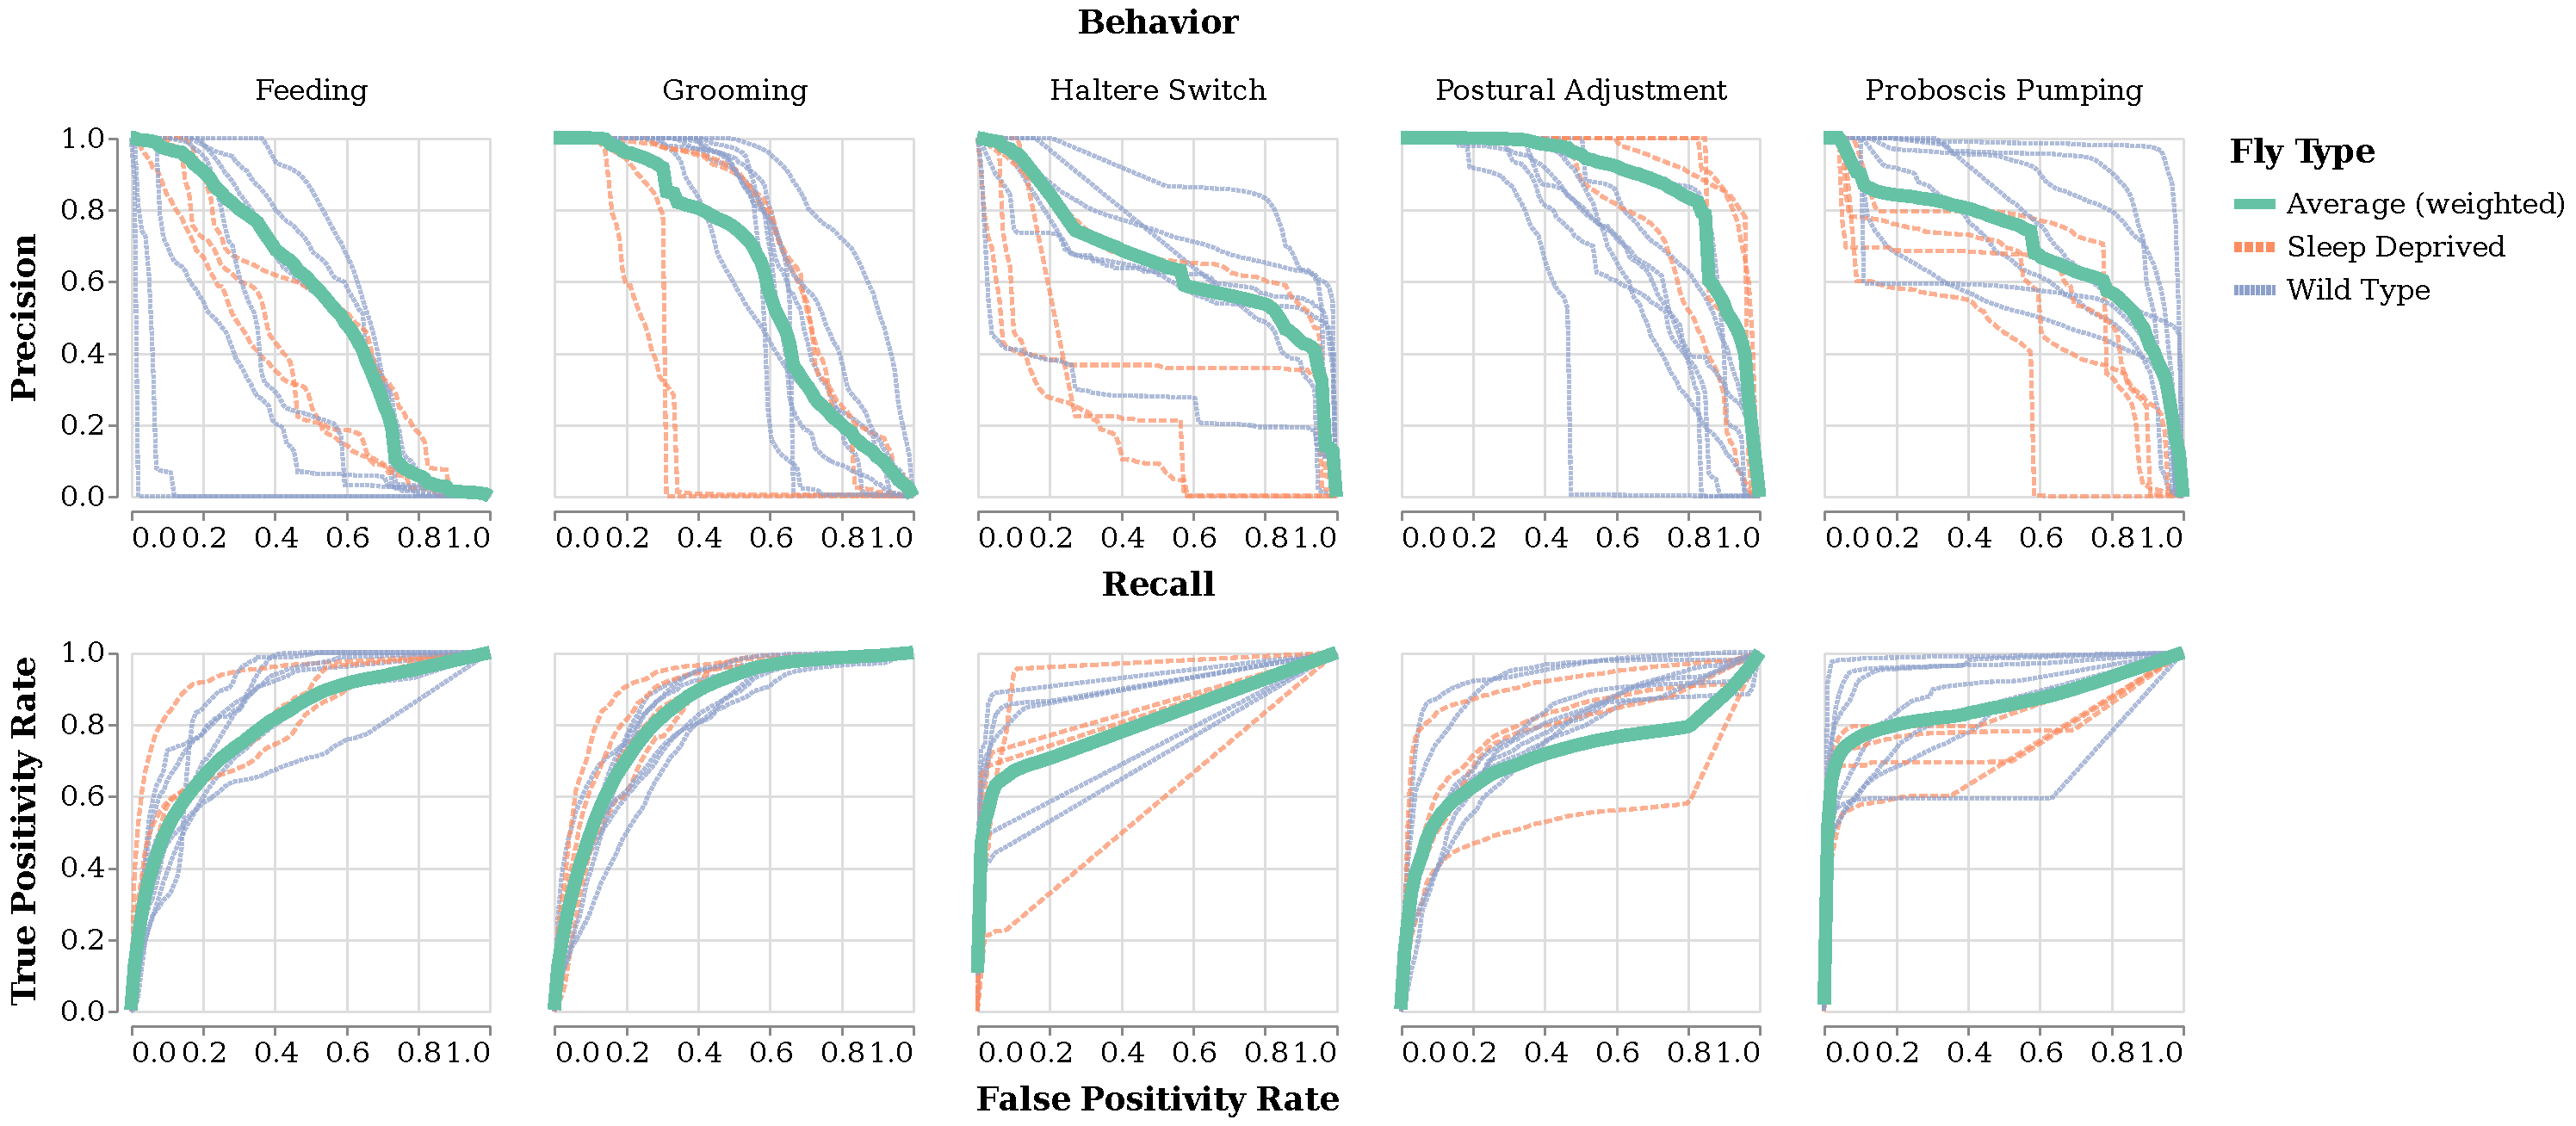
\includegraphics[width=\linewidth]{figures/PRC_ROC-DAnnfiltered.pdf}
		\caption{ROC and precision-recall curves for annotated frames. \label{figure:ROC-PRC-Ann}}
	\end{subfigure}%
	\caption[Performance summary of behavior mapping demonstrated using receiver operating characteristic curve and precision-recall curve.
	]{Performance summary of behavior mapping demonstrated using receiver operating characteristic curve and precision-recall curve.
		Weighted average of ROC and precision-recall curves computed by interpolation.
		Curves for both frames estimated as micro-activity and annotated frames are given respectively in Figures~\ref{figure:ROC-PRC-Act}, ~\ref{figure:ROC-PRC-Ann}. \label{figure:ROC-PRC}}
\end{figure}

\begin{figure}[htb!]
	\centering
	\begin{subfigure}[b]{0.5\linewidth}
		\centering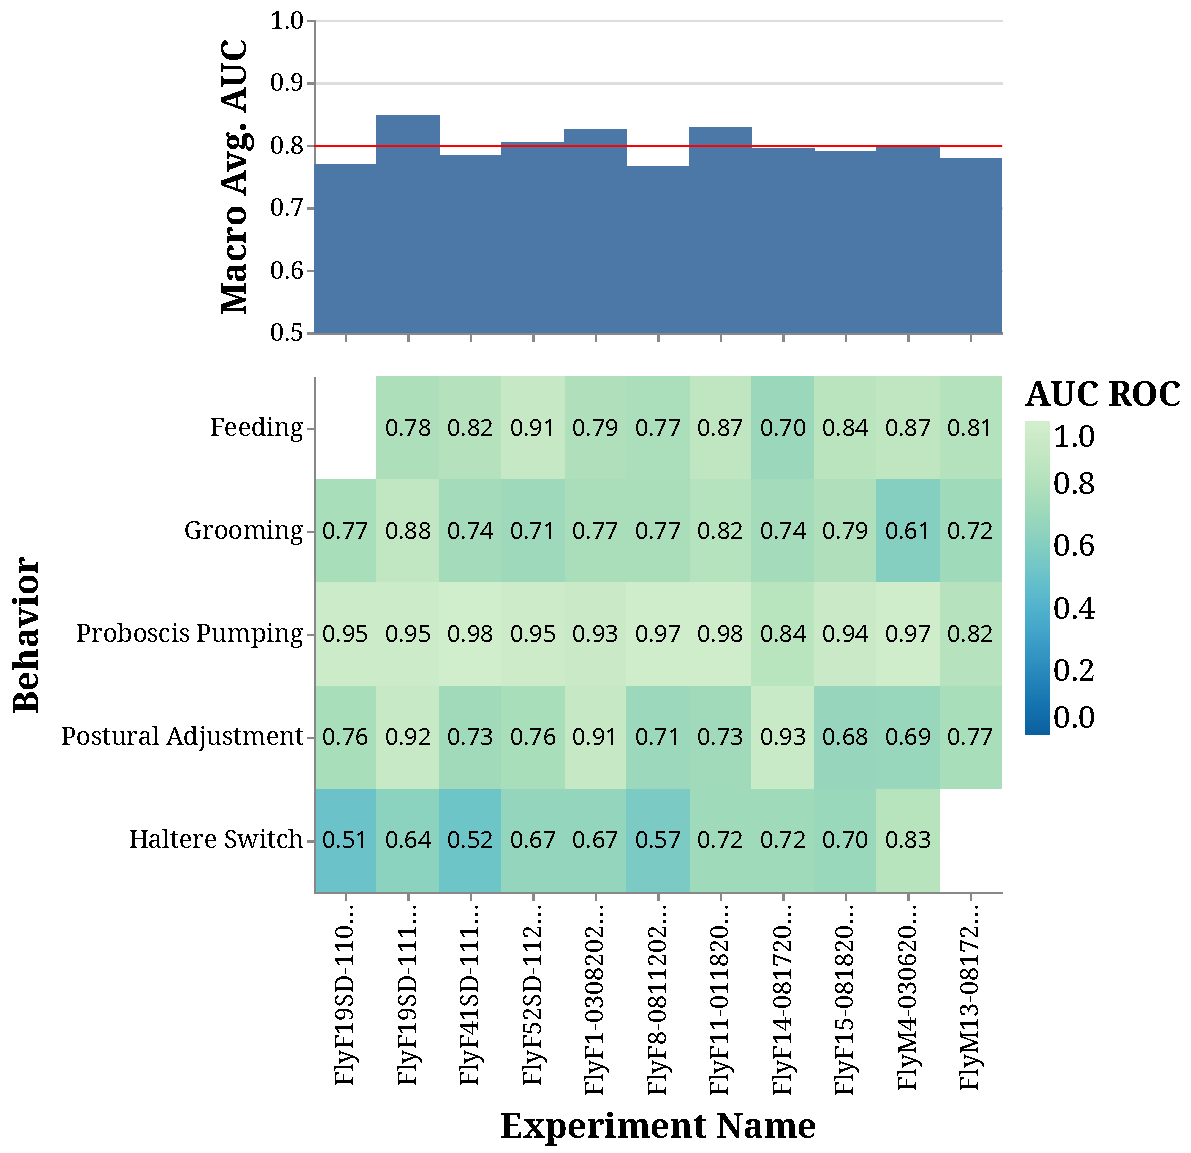
\includegraphics[width=\linewidth]{figures/AUC_ROC-DActfiltered.pdf}
		\caption{AUC scores for $\MicroActivity$ set. \label{figure:AUC-ROC-Act}}
	\end{subfigure}%
	\hfill
	\begin{subfigure}[b]{0.5\linewidth}
		\centering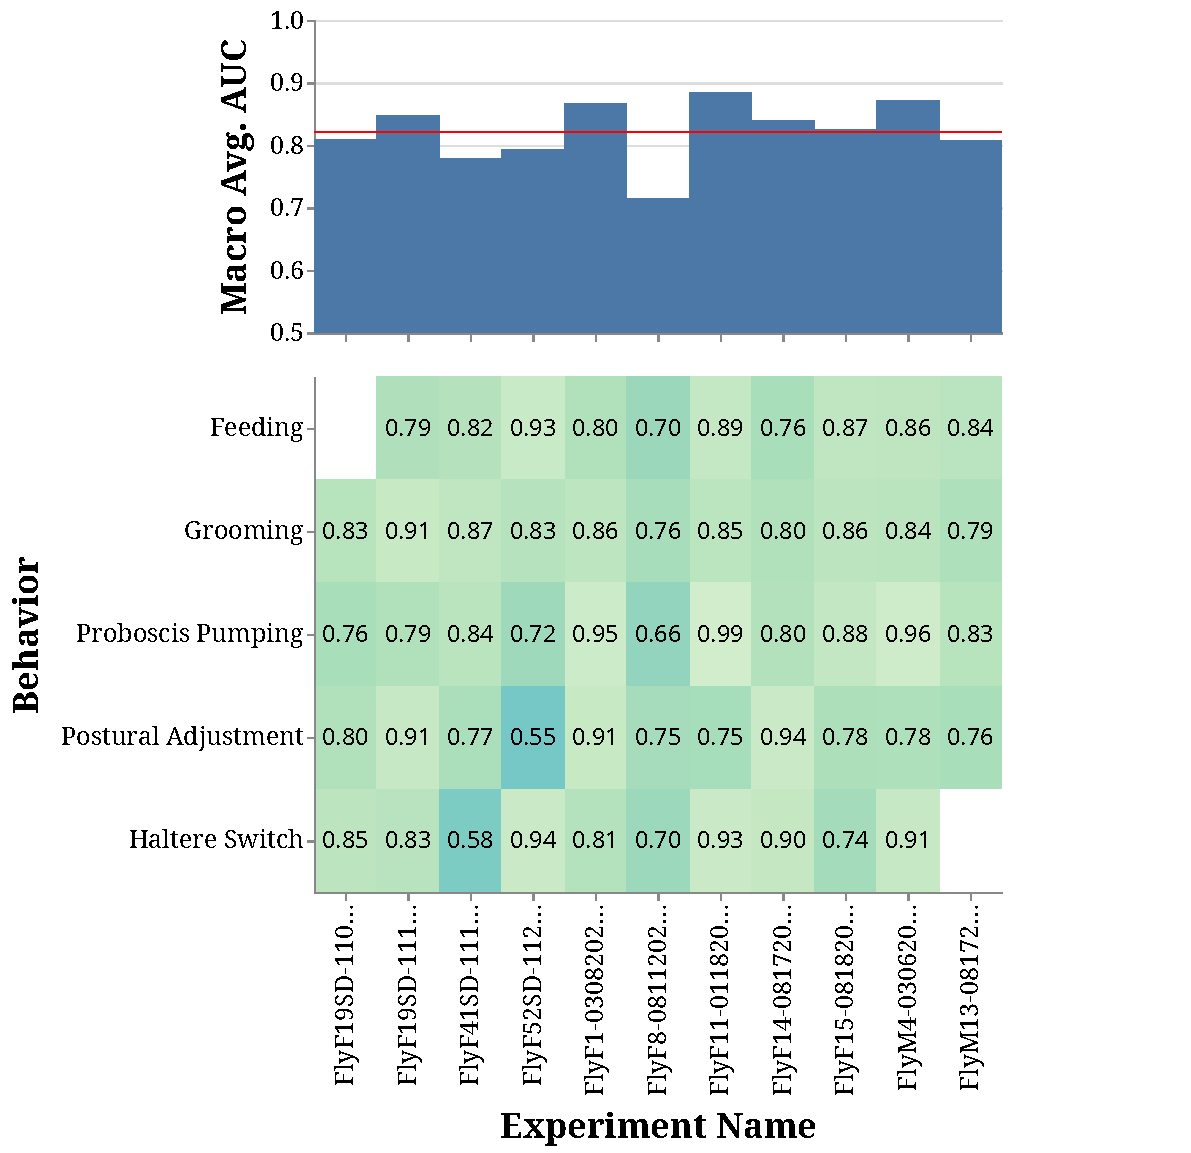
\includegraphics[width=\linewidth]{figures/AUC_ROC-DAnnfiltered.pdf}
		\caption{AUC scores for annotated frames. \label{figure:AUC-ROC-Ann}}
	\end{subfigure}%
	\caption[Performance summary of behavior mapping with area under curve scores of ROC.]
	{Performance summary of behavior mapping with area under curve scores of ROC.
		The red line indicates the macro average of AUC scores for each split.
		Scores for both frames estimated as micro-activity and annotated frames are given respectively in Figures~\ref{figure:AUC-ROC-Act}, ~\ref{figure:AUC-ROC-Ann}.
		\label{figure:AUC}}

\end{figure}

Using behavioral computed behavioral scores, we computed precision recall and receiver operating characteristic curves for each split, and also computed interpreted weighted averages of curves, see Figure~\ref{figure:ROC-PRC} and Figure~\ref{figure:AUC}.
Evaluations are done by considering two subsets of frames, the first subset is the frames annotated as one of the behavioral categories and the other one is the $\MicroActivity$ set.
The latter one contains false positive micro-activity frames, which is quantified as the recall score of quiescent and other category.
False positive micro-activity frames affects haltere switch detection performance most, for instance, its weighted mean precision decreases by ${\sim}0.5$ for fixed recall at ${\sim}0.65$.
This performance difference also shows the importance of achieving low recall for quiescent and other category in the experiment outlining stage.
Since the evaluation is done with the $\MicroActivity$ set is more realistic, the following comments are made on considering it.

The most robust detection is achieved for proboscis pumping and postural adjustment behavioral categories, respectively achieving $\textnormal{F-}1$ greater than $0.8$ and $0.85$ scores for some splits.
The maximum $\textnormal{F-}1$ score achieved for grooming is $0.60$ for FlyF1-03082020164520 split, whereas $\textnormal{F-}1$ of haltere switch behavioral category do not exceed $0.4$.
AUC scores for the proboscis pumping often exceeds $0.95$, implying robust detection for almost all the splits.
We observe that detection performance vary greatly among different experiments. This variation can be due to a number of reasons, but most likely reasons are related to tracking performance and annotation quality, and as well as behavioral repertoires of flies.
Considering all splits together, we achieve a macro average of $0.8$ AUC score with a one-versus-rest approach.

As discussed in the Chapter~\ref{chapter:introduction}, the behavioral repertoire of the fruit fly is much richer than the behavioral categories that we considered.
Moreover, there exists a great amount of variation among flies behavioral repertoire and behavioral visits (see Section~\ref{section:analyzing-behavioral-repertoire}).
Thus, we also investigate our pipeline's ability of detection of unseen behavioral categories by utilizing behavioral scores.
Such an ability is important for avoiding misleading the user of the pipeline. It may also be desired to reconsider defined and annotated behavioral categories, and may further lead to interesting biological observations.
To this end, we consider the following experimental setting: behavior mapping of an unannotated experiment (FlyF1-03082020) is done separately for two annotated experiments, namely FlyF14-0817202 and FlyM13-08172021.
Then, behavioral scores of the FlyF1-03082020's frames with haltere switch annotation is compared between FlyF14-0817202 guided mapping and FlyM13-08172021 guided mapping.
As it can be seen from the Figure~\ref{figure:time-spent-in-behaviors}, FlyF1-03082020 and FlyF14-0817202 spent ${\sim}4$ minutes by exhibiting switch like haltere movement behavior, whereas FlyM13-08172021 spent no more than $5$ seconds.
Therefore, compared to FlyF14-0817202, haltere switch is an unseen and lacking behavioral category for FlyM13-08172021.
We expect to identify this using behavioral scores.
Indeed, behavioral scores reflect the difference in the behavioral repertoires of the annotated flies.
As it can be seen in the Figure~\ref{figure:repertoire-score-comparison}, behavioral scores obtained based on FlyF14-0817202's behavioral repertoire are much more confident about the correct behavioral category, whereas behavioral scores obtained based on FlyM13-08172021's behavioral repertoire are more uniform-like and total score is often shared among multiple behavioral categories.
Using the entropy of the behavioral score, one can quantify existing of unseen and new behavioral categories in a more systematic way.
In the Figure~\ref{figure:repertoire-entropy-comparison}, we compare entropy distributions of the behavioral scores obtained using annotated experiments FlyM13-08172021 and FlyF14-0817202.
We can immediately see that scores obtained based on the FlyM13-08172021's repertoire have higher entropy, with mean $0.41$, whereas for the other one mean is $0.15$.
For instance, if the entropy of a frame's score is greater than $0.2$, it may be recommended to visit them and investigate the reason.
Accordingly, extending or re-considering behavioral annotations can be necessary.

\begin{figure}[hbt!]
	\centering
	\begin{subfigure}[b]{0.55\linewidth}
		\centering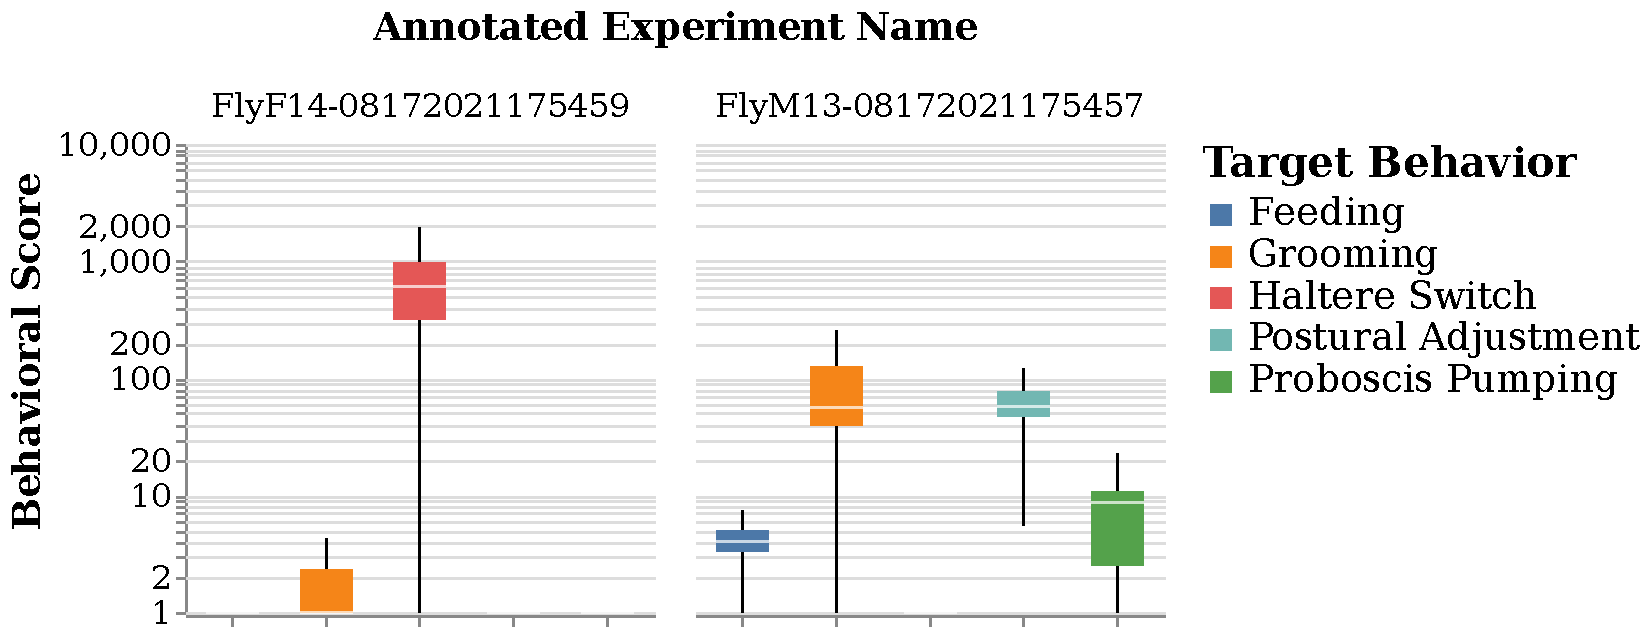
\includegraphics[width=\linewidth]{figures/BehavioralScores-RepertoireDifference.pdf}
		\caption{Behavioral score values, before $\textnormal{L-}1$ normalization. \label{figure:repertoire-score-comparison}}
	\end{subfigure}%
	\centering
	\begin{subfigure}[b]{0.45\linewidth}
		\centering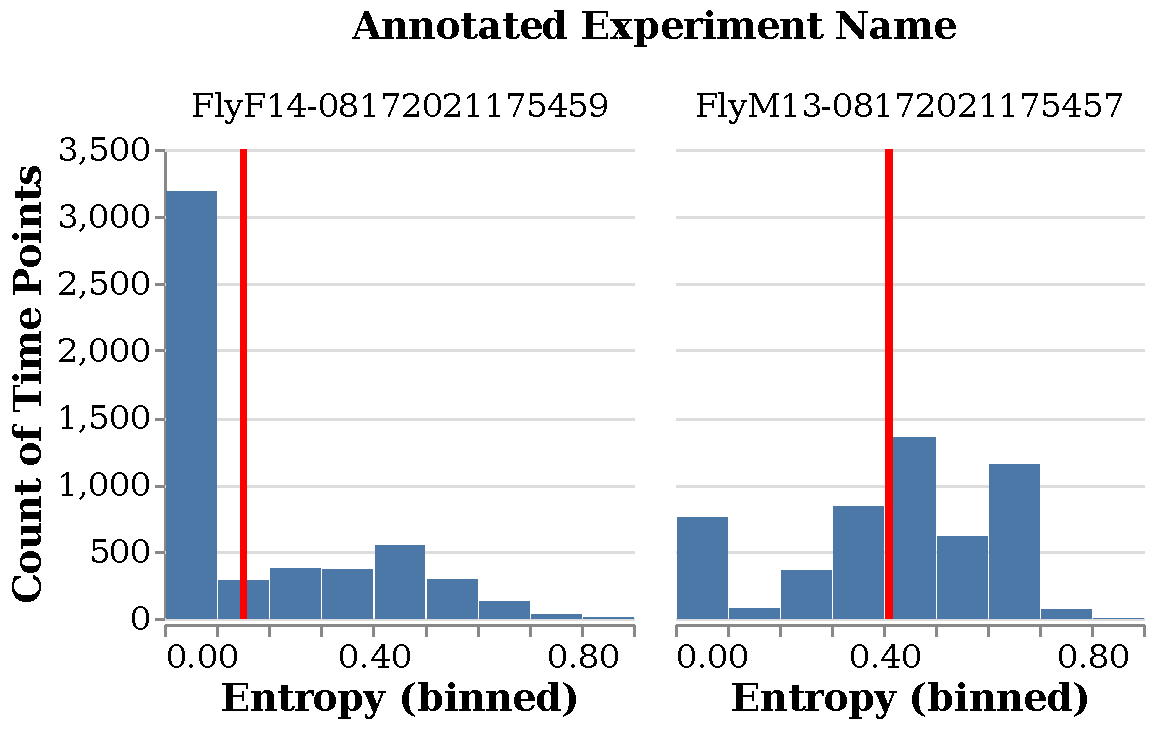
\includegraphics[width=\linewidth]{figures/Entropy-RepertoireDifference.pdf}
		\caption{Entropy values. The red line, is the mean. \label{figure:repertoire-entropy-comparison}}
	\end{subfigure}%
	\caption[Histogram of entropy values and box-plot of the behavioral scores computed using one unannotated and two annotated experiments with varying behavioral repertoires.]{Histogram of entropy values and box-plot of behavioral scores computed using one unannotated and two annotated experiments with varying behavioral repertoires.
		Here, behavioral repertoire of FlyF1-03082020 is predicted separately with two different annotated experiments, namely FlyF14-08172021 and FlyM13-08172021.
		Behavioral scores and entropy values are computed for the haltere switch behavior.
		The latter one lacks the haltere switch behavior, and as a result behavioral scores tend to have higher entropy.
		Results demonstrate the ability of the proposed pipeline to detect and discover unseen unannotated behavioral categories using behavioral scores.\label{figure:repertoire-difference}}
\end{figure}

\section{Analyzing Behavioral Repertoire}\label{section:analyzing-behavioral-repertoire}
In this section, we analyze the collected data of sleep experiments to discover how behaviors that we are interested in exhibited.
Starting from a broad perspective, the most brief description of sleep experiments can be done by quantifying the displacement of the flies placed in the chamber.
In the Figure~\ref{figure:displacement}, we plot velocity-based feature vectors $\V{u}$ between ZT10-ZT02 and ZT10-ZT06, respectively for each wild type sleep and sleep-deprived experiments.
We observe that the long dormancy epochs are interrupted by relatively short macro activity bouts during the sleep.
In addition to short macro activity bouts, we observe very small displacements all over the night, which indicates there exists micro-activities other than major positional and postural changes.
Hence, a more fine-grained analysis and closer look is necessary, as this work attempts to achieve.

\begin{figure}[htb!]
	\centering
	\begin{subfigure}[ht!]{0.95\linewidth}
		\centering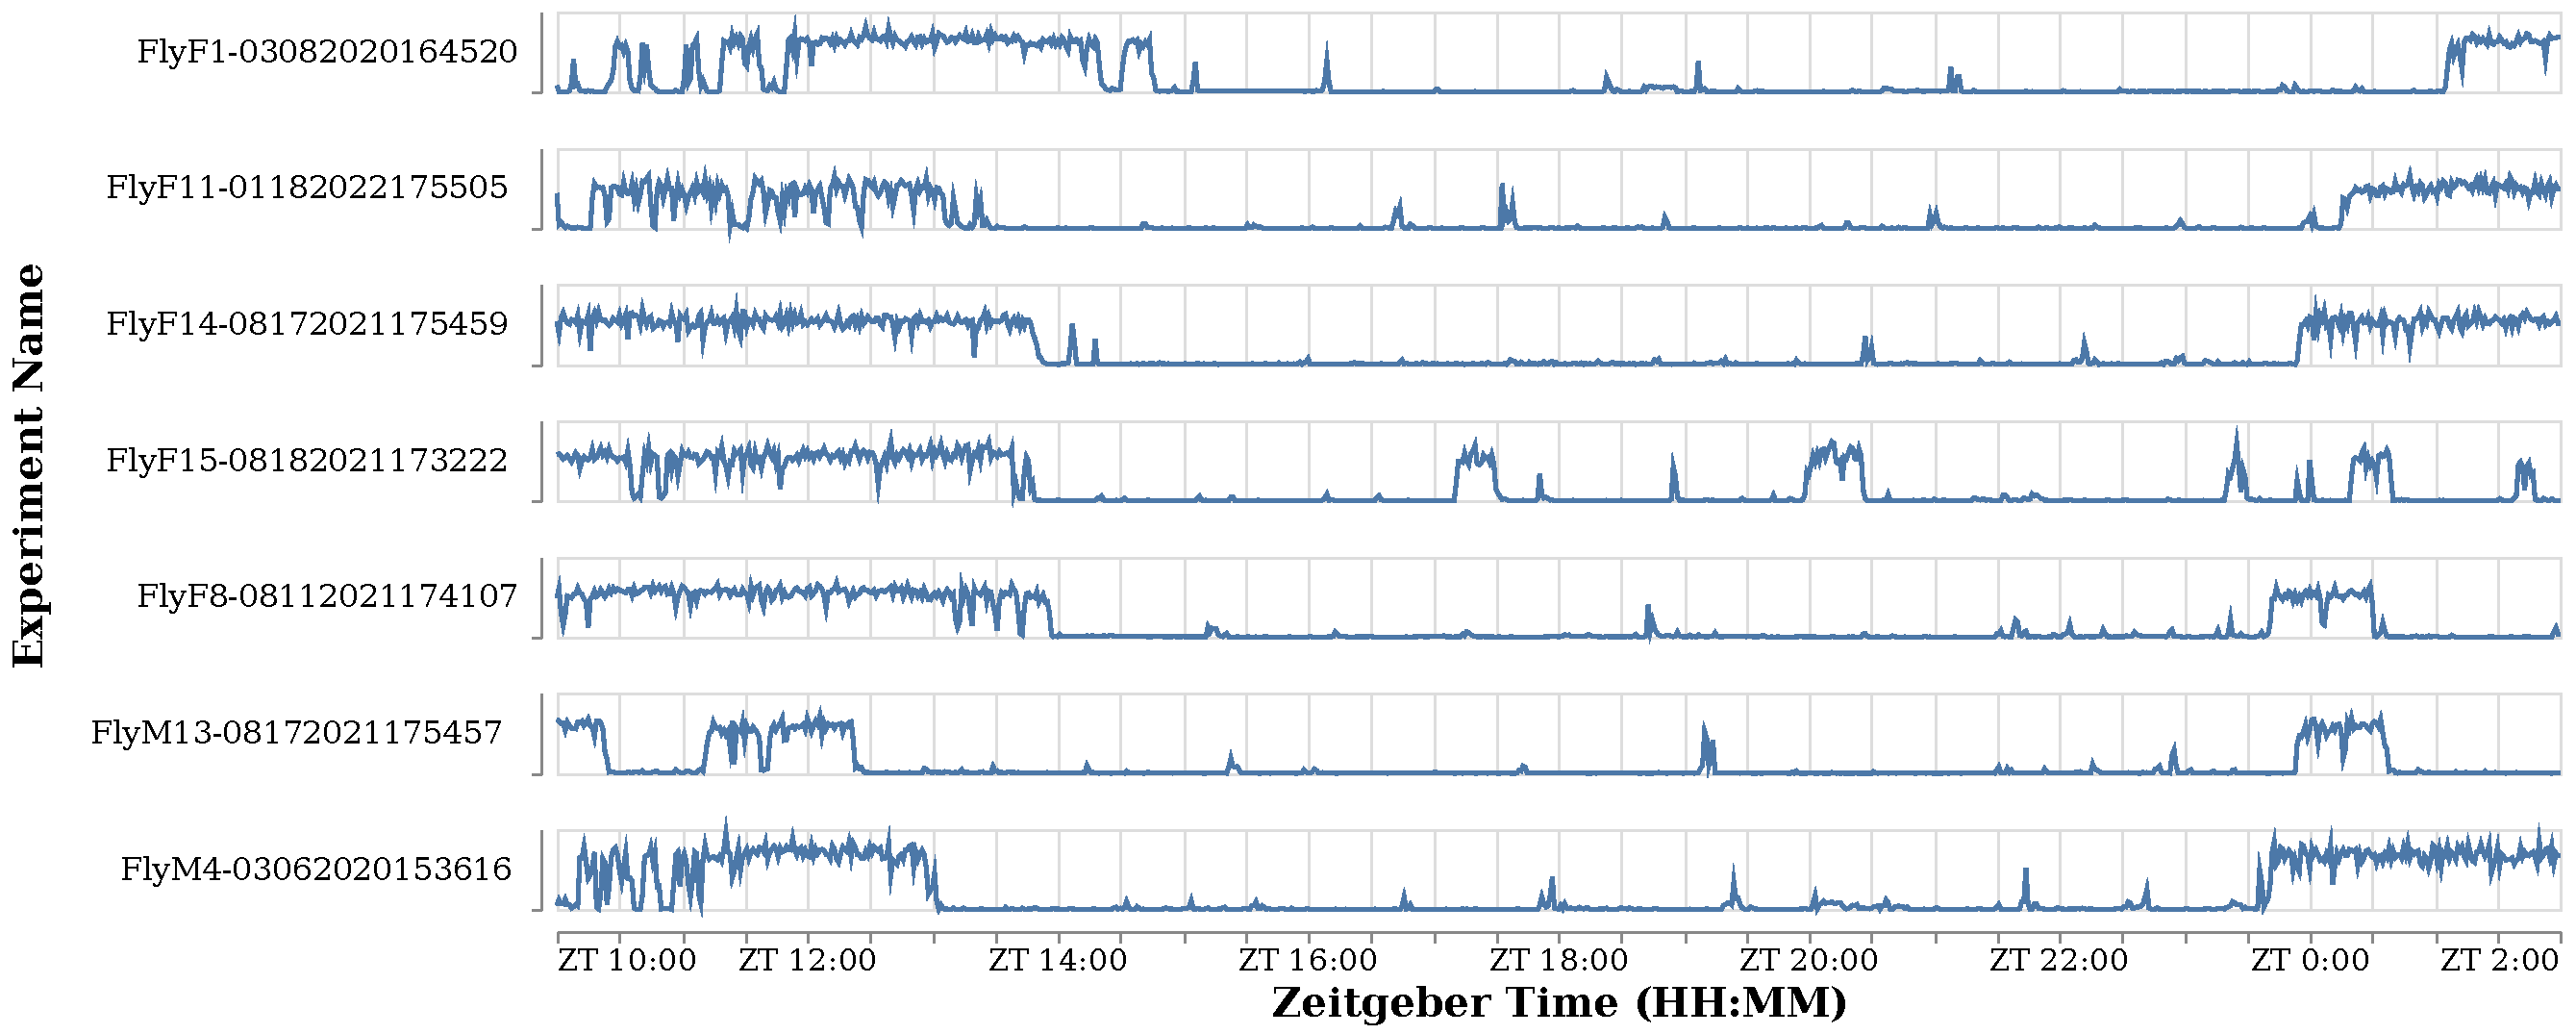
\includegraphics[width=\linewidth]{figures/Velocity-WT-1T.pdf}
		\caption{Wild type.}
	\end{subfigure}%

	\begin{subfigure}[ht!]{0.95\linewidth}
		\centering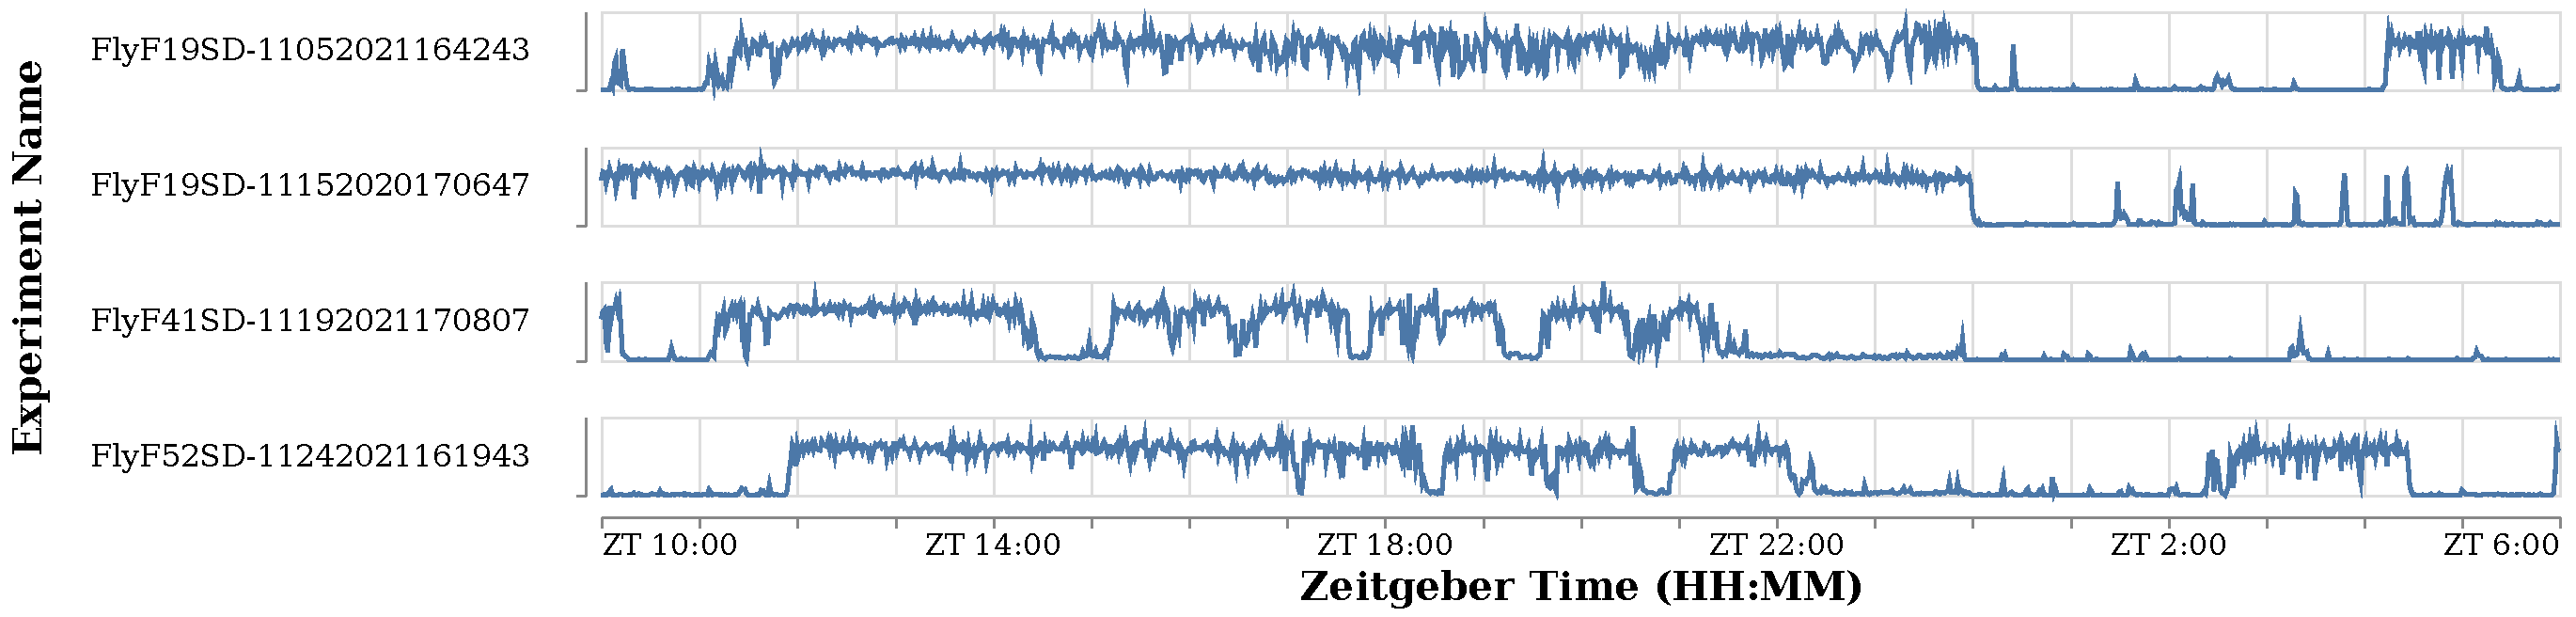
\includegraphics[width=\linewidth]{figures/Velocity-SD-1T.pdf}
		\caption{Sleep deprived.}
	\end{subfigure}%
	\caption[Overall displacement values over entire experiments.]{Overall displacement values over entire experiments.
		Displacement of the body reveals long dormancy and sleep epochs, and macro-activities.
		Displacement values are computed as described in Equation~\ref{equation:displacement}, and smoothed with a rolling mean of 1-minute window.\label{figure:displacement}}
\end{figure}

In the Figure~\ref{figure:heatmap-microactivity}.

\begin{figure}[htb!]
	\centering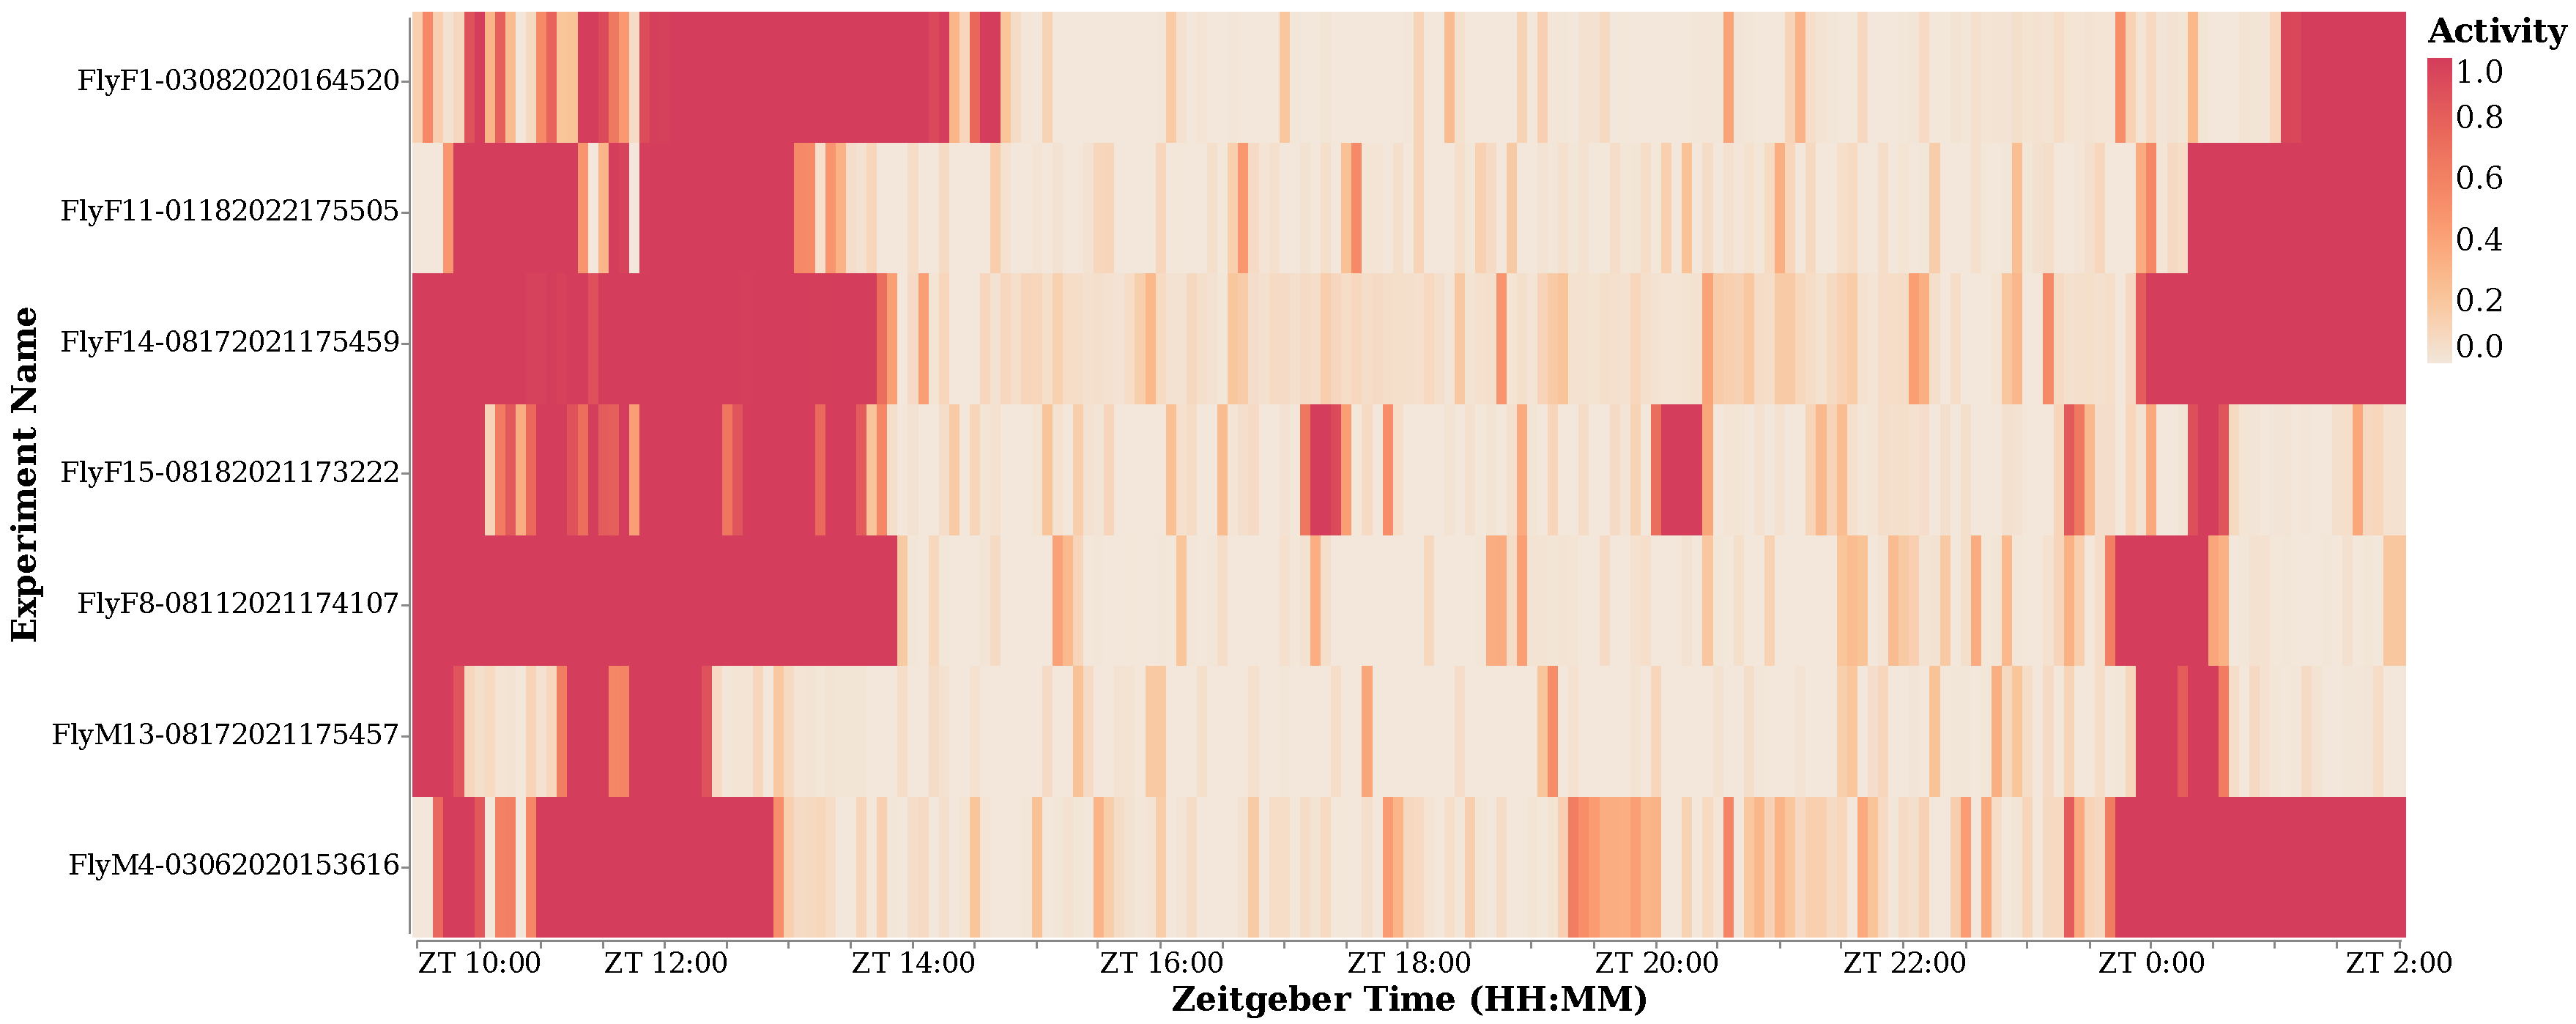
\includegraphics[width=\linewidth]{figures/ActivityBinned-Ann-WT-5T.pdf}
	\caption[Binned temporal heatmap of activities.]{Binned temporal heatmap of activities.
		Each bin is $5$ minutes, corresponding to $900$ frames.
		Activity value is computed as the ratio of the number of annotated frames and total number of frames in that bin. \label{figure:heatmap-microactivity}}
\end{figure}

In the Figure~\ref{figure:summary-behavior-characteristics}.

\begin{figure}[htb!]
	\centering
	\begin{subfigure}[b]{0.95\linewidth}
		\centering
		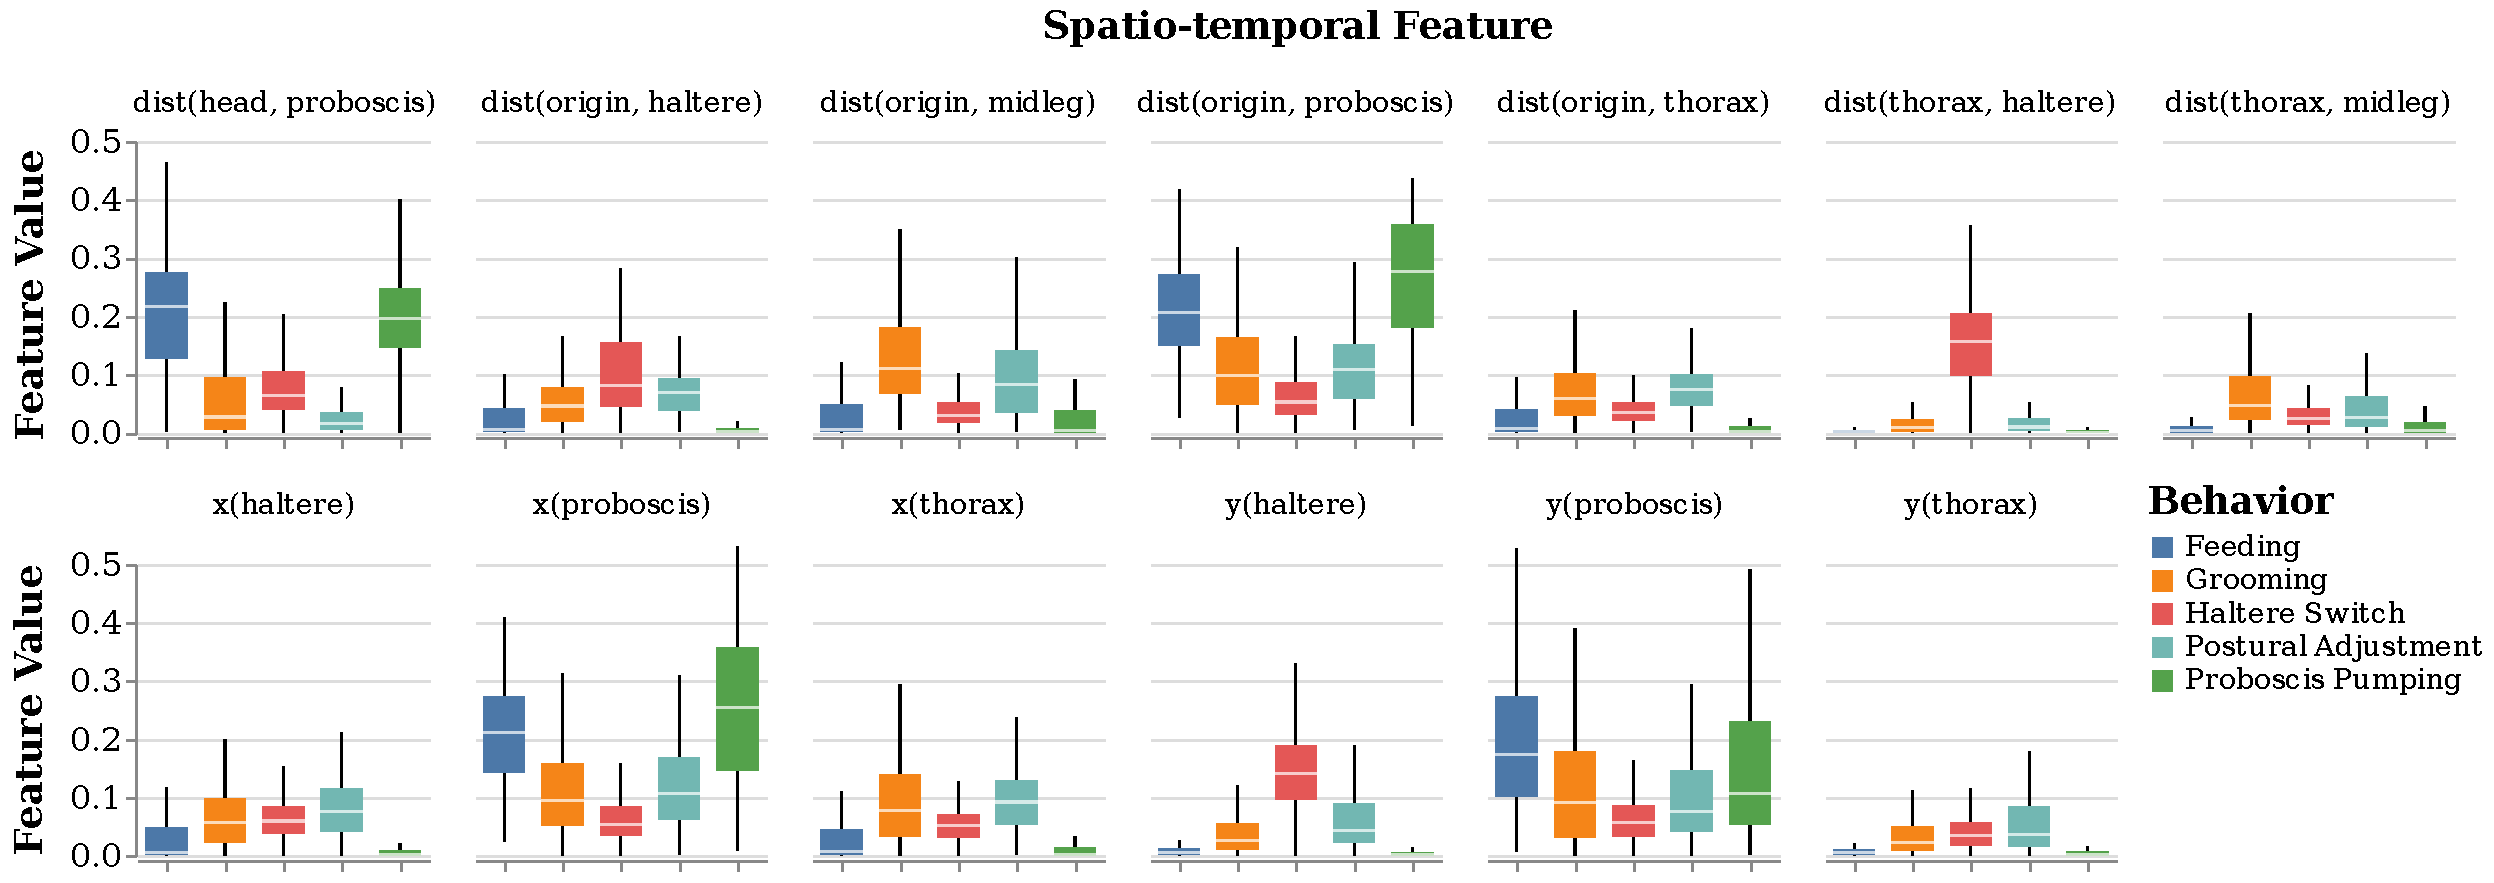
\includegraphics[width=\linewidth]{figures/FeatureDistributions_perBehavior-Ann.pdf}
		\caption{Summation of all frequency channels of behavioral representation value for each spatio-temporal feature.}
	\end{subfigure}%

	\centering
	\begin{subfigure}[b]{0.95\linewidth}
		\centering
		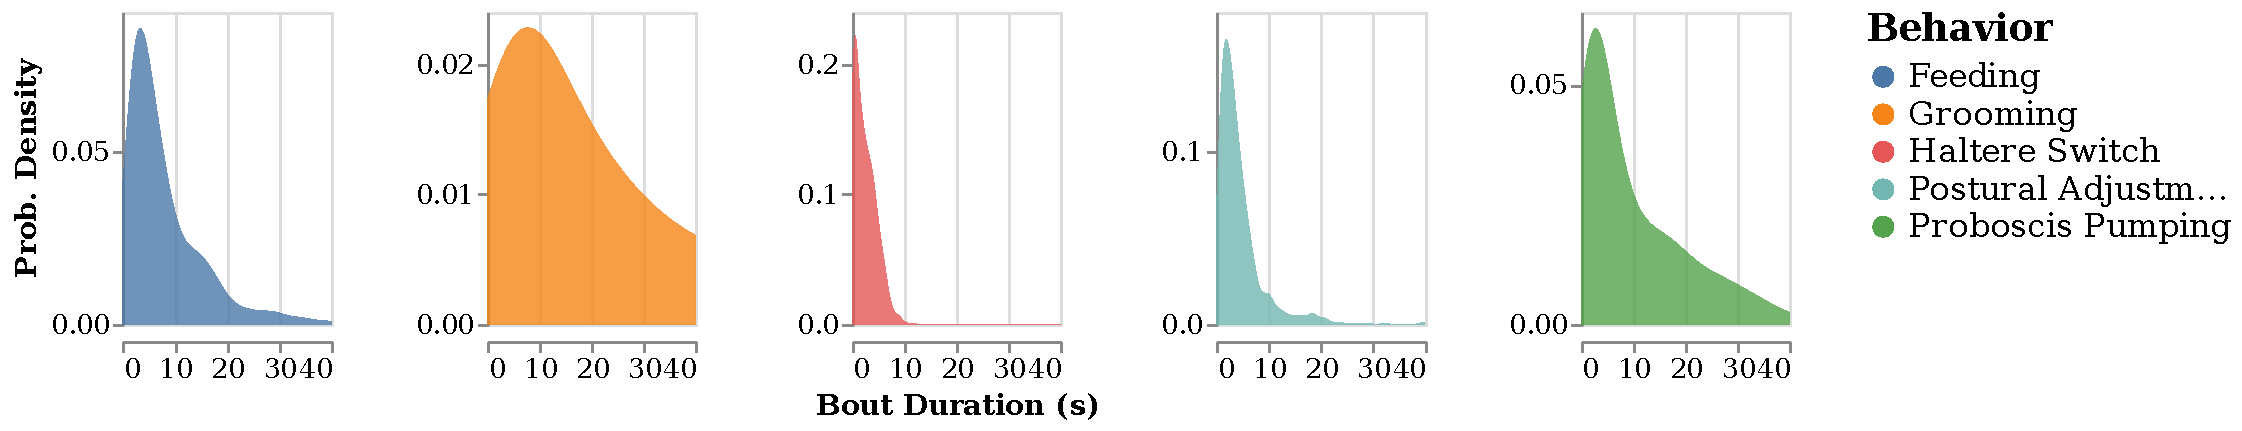
\includegraphics[width=\linewidth]{figures/BoutDurationDistributions-Ann.pdf}
		\caption{Kernel density estimations of bout durations for each behavioral category. Variance of bout durations within and across behavioral categories demonstrates the rich behavioral repertoire.}
	\end{subfigure}%

	\centering
	\begin{subfigure}[htb!]{0.95\linewidth}
		\centering
		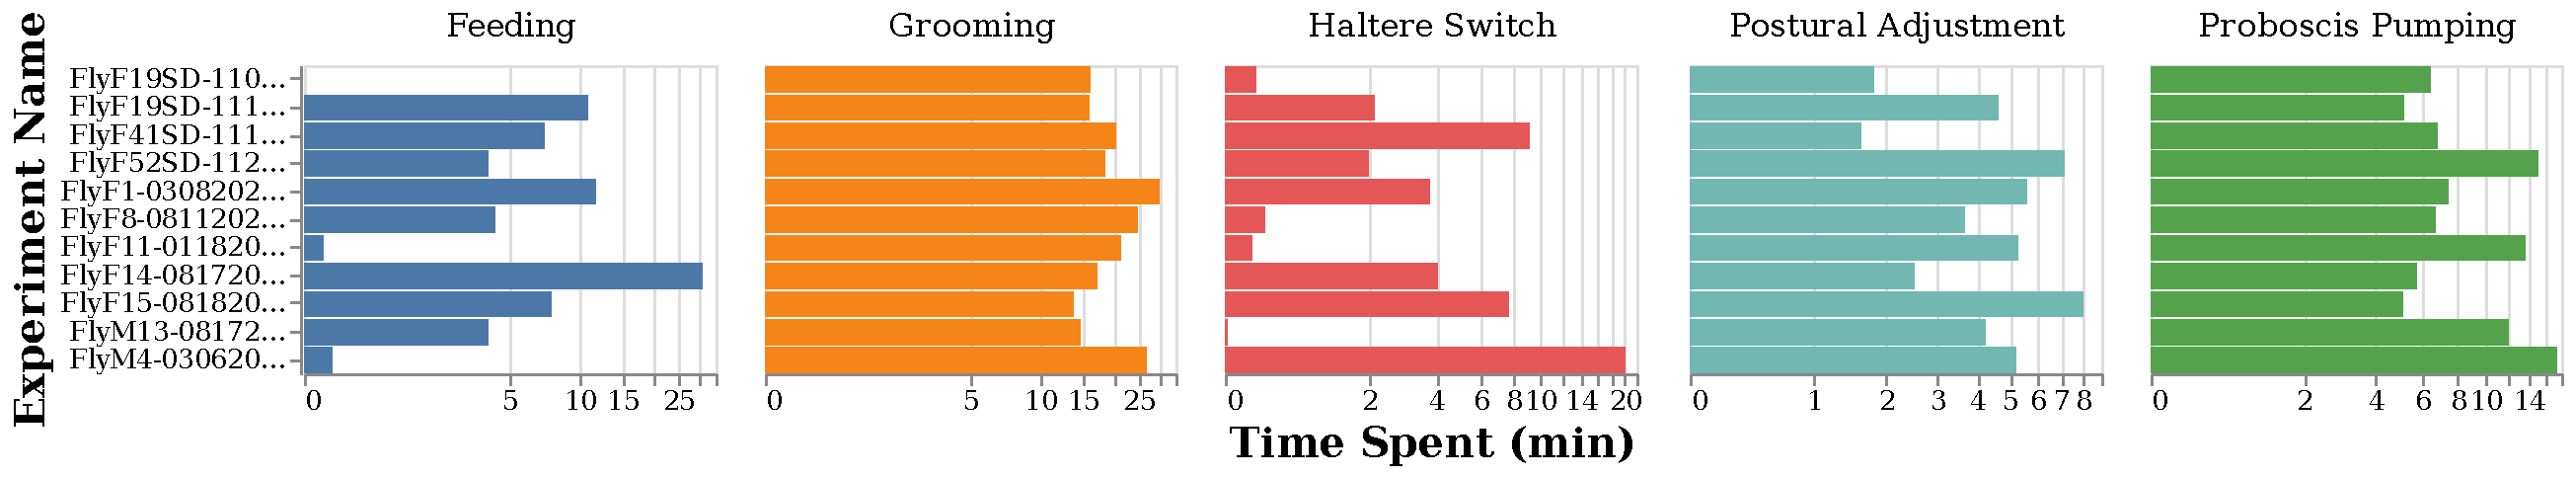
\includegraphics[width=\linewidth]{figures/TimeSpent-perBehavior-Ann.pdf}
		\caption{Time spent with each behavioral category for all experiments. \label{figure:time-spent-in-behaviors}}
	\end{subfigure}%
	\caption{Summary of behavioral repertoires of different fly, demonstrated using both spatial and temporal characteristics. \label{figure:summary-behavior-characteristics}}
\end{figure}

In the Figure~\ref{figure:temporal-organization-behavior}.

\begin{figure}[htb!]
	\centering
	\begin{subfigure}[b]{0.975\linewidth}
		\centering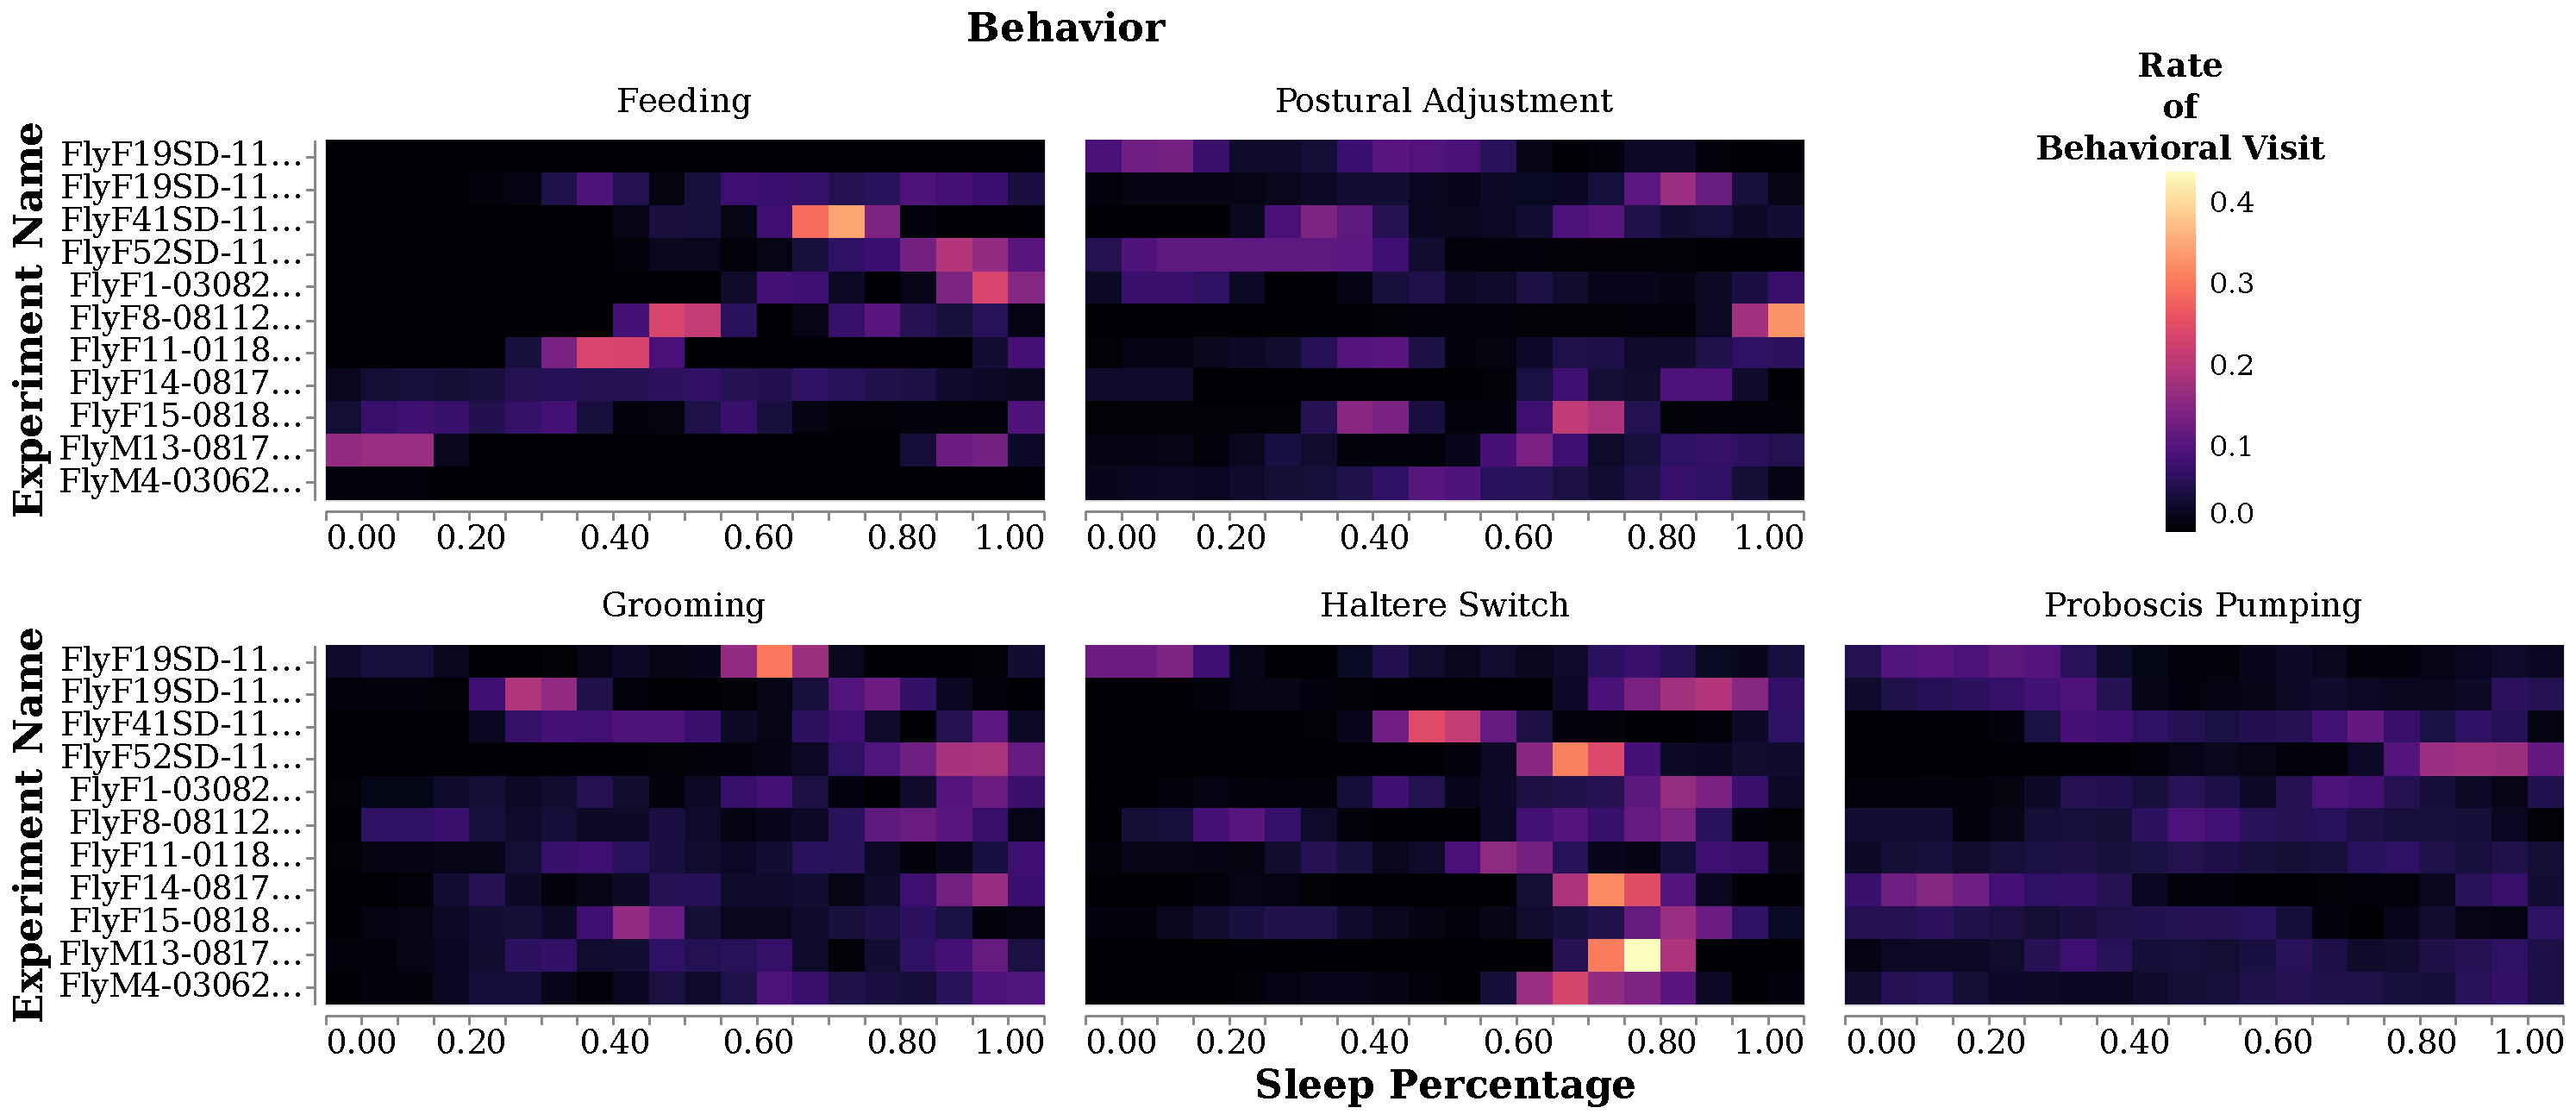
\includegraphics[width=\linewidth]{figures/Heatmap_BehavioralUsage-Ann.pdf}
		\caption{Rate of behavioral visits during the sleep within each $0.05$ sleep percentage bin. Each row is normalized to sum up to $1$.}
	\end{subfigure}%

	\centering
	\begin{subfigure}[b]{0.975\linewidth}
		\centering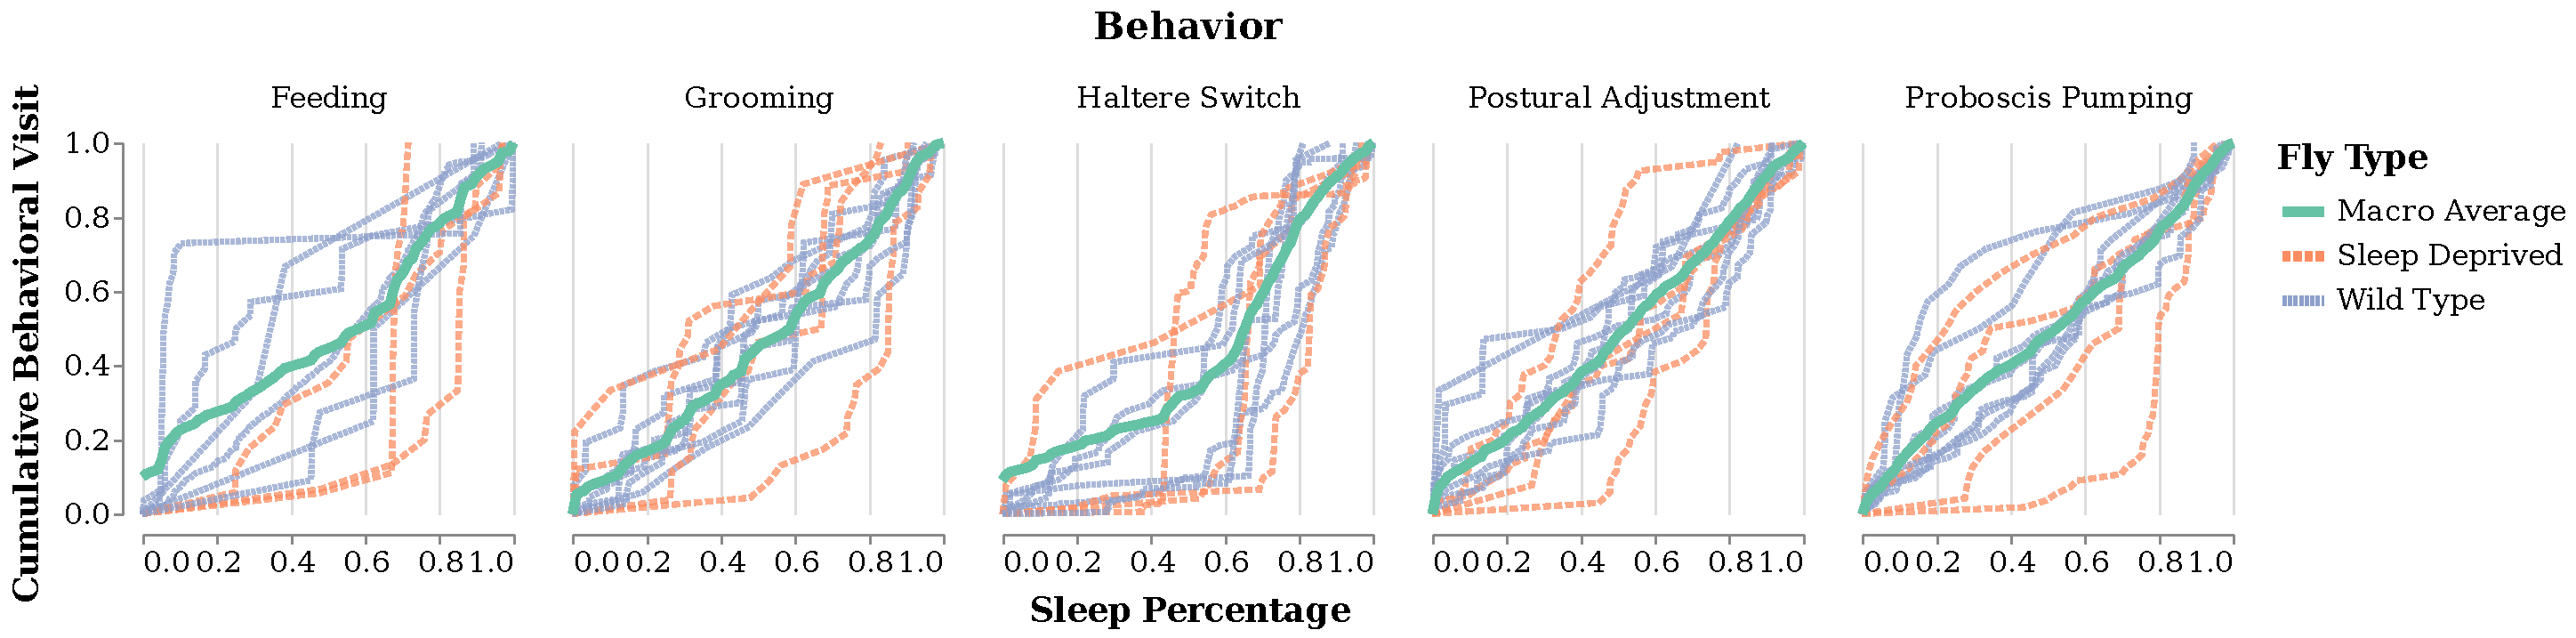
\includegraphics[width=\linewidth]{figures/CumulativeLine_BehavioralUsage-Ann.pdf}
		\centering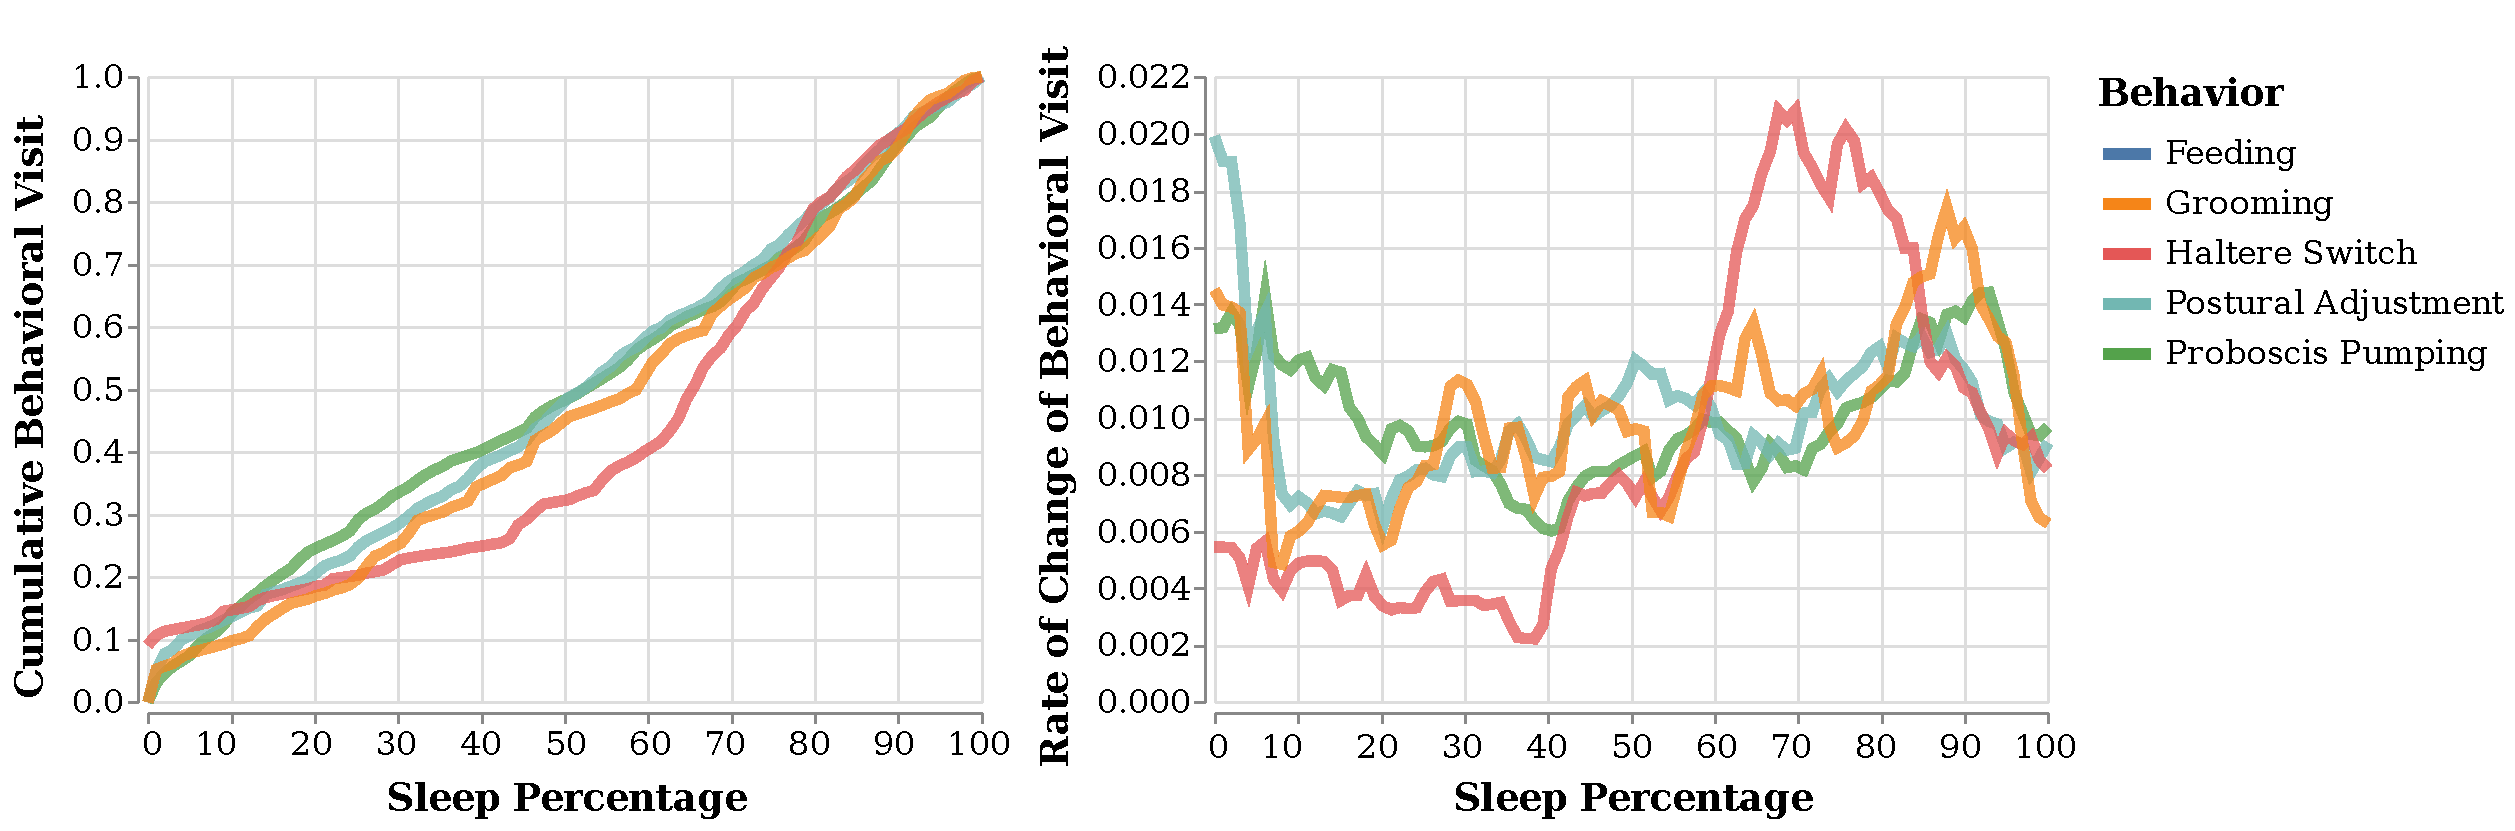
\includegraphics[width=\linewidth]{figures/MeanCumRofC_BehavioralUsage-Ann.pdf}
		\caption{Cumulative behavioral visits for each behavior, behaviors with less than 2 bouts are excluded.}
	\end{subfigure}%

	\caption[Demonstration of behavioral visits during the sleep.]{Demonstration of behavioral visits during the sleep.
		Ethograms of flies are aligned by dividing the longest dormant epoch to $100$ bin, corresponding to the sleep percentages.
		Number of behavioral visits are normalized by the total number of bouts for each fly and behavioral category, separately. \label{figure:temporal-organization-behavior}}

	% \centering
	% \begin{subfigure}[b]{0.45\linewidth}
	% 	\centering
	% 	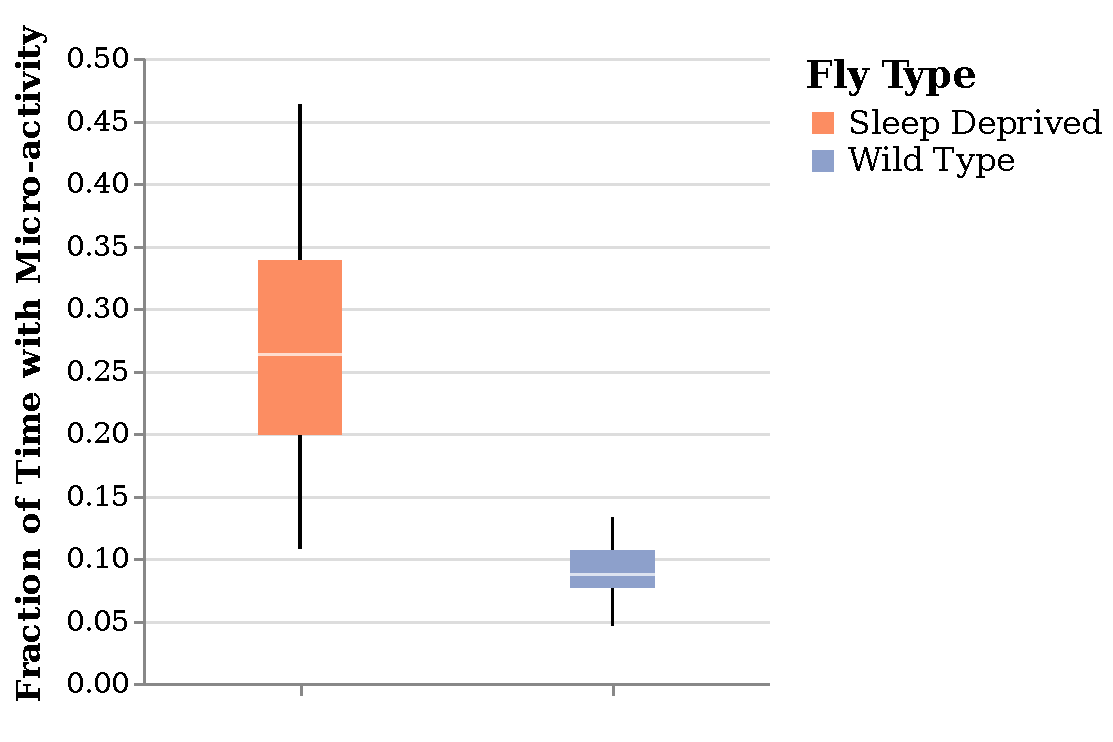
\includegraphics[width=\linewidth]{figures/FractionTime-Microactivity.pdf}
	% 	\caption{Fraction of time spent with micro-activities in dormant epochs, comparing wild type experiments and sleep deprived experiments.}
	% \end{subfigure}%
\end{figure}
